% Use the following line _only_ if you're still using LaTeX 2.09.
%\documentstyle[icml2015,epsf,natbib]{article}
% If you rely on Latex2e packages, like most moden people use this:
\documentclass{article}

% use Times
\usepackage{times}
% For figures
\usepackage{graphicx} % more modern
%\usepackage{epsfig} % less modern
\usepackage{subfigure} 

% For citations
\usepackage{natbib}

% For algorithms
% \usepackage{algorithm}
% \usepackage{algorithmic}

% As of 2011, we use the hyperref package to produce hyperlinks in the
% resulting PDF.  If this breaks your system, please commend out the
% following usepackage line and replace \usepackage{icml2015} with
% \usepackage[nohyperref]{icml2015} above.
\usepackage{hyperref}

% Packages hyperref and algorithmic misbehave sometimes.  We can fix
% this with the following command.
% \newcommand{\theHalgorithm}{\arabic{algorithm}}

% Employ the following version of the ``usepackage'' statement for
% submitting the draft version of the paper for review.  This will set
% the note in the first column to ``Under review.  Do not distribute.''
% \usepackage{icml2015} 

% Employ this version of the ``usepackage'' statement after the paper has
% been accepted, when creating the final version.  This will set the
% note in the first column to ``Proceedings of the...''
\usepackage[accepted]{icml2015}

\usepackage{cleveref}

% The \icmltitle you define below is probably too long as a header.
% Therefore, a short form for the running title is supplied here:
\icmltitlerunning{Group 2 Update 2}

\begin{document} 
\twocolumn[
\icmltitle{Group 2 Update 2: United States Obesity Risk Factor Data Analysis}

% It is OKAY to include author information, even for blind
% submissions: the style file will automatically remove it for you
% unless you've provided the [accepted] option to the icml2015
% package.
\icmlauthor{Brian Desnoyers}{bdesnoy@ccs.neu.edu}
%\icmladdress{Your Fantastic Institute,
%            314159 Pi St., Palo Alto, CA 94306 USA}
\icmlauthor{Alankrit Joshi}{alankrit93@ccs.neu.edu}
\icmlauthor{Rahul Kondakrindi}{rahulkondakrindi@ccs.neu.edu}
\icmlauthor{Prasanna Vikash Peddinti}{vikash4281@ccs.neu.edu}
\icmlauthor{Junyi Wang}{wang4615@ccs.neu.edu}

% You may provide any keywords that you 
% find helpful for describing your paper; these are used to populate 
% the "keywords" metadata in the PDF but will not be shown in the document
%\icmlkeywords{boring formatting information, machine learning, ICML}

\vskip 0.3in
]

% \begin{abstract} 
% \end{abstract} 

\section{Introduction and Dataset}
\label{introduction}

Obesity is a major challenge facing the healthcare system in the United States. Obesity rates have risen significantly over the last thirty years and if this trend continues, the United States healthcare system is projected to pay \$150 billion annually \cite{hurt2010obesity}.
In addition to genetic factors, this increase in obesity rates, inactivity, and malnutrition has been linked to the environment. 
Environmental changes; such as car transportation, inactive jobs, carry out food, food advertisements, and food portions; can be tied to specific regions and have a significant impact on health \cite{whyobesityhealthproblem, understandingadultoverweight}. 
The main goal of this project is to explore the distribution of these risk factors across the United States and visualize how these groupings correspond to obesity and health.
\\\\
For this project, we will analyze the Nutrition, Physical Activity, and Obesity dataset provided by the Centers for Disease Control and Prevention (CDC).
This dataset provides information on the percentage of the population suffering from adult obesity, as well as associated behaviors, such as poor nutrition and physical inactivity, for the nation, states, and selected sub-state districts. 
These data also include potential risk factor features, such as age, education, sex, and income \cite{nutphysactobesitydata}.
In addition, this dataset provides similar population information for child obesity, infant breastfeeding, active transportation, and community policy supports.

\section{Preprocessing}
\label{preprocessing}
The main purpose of our team's work for this update was driven around exploratory analysis, which started with data pre-processing. Since the dataset from the CSV was available in CSV format, it was easy to read without file format conversion. After reading in the dataset, we focused on understanding each column to allow us to extract the columns useful for our analysis. 
\\\\
Unfortunately the raw dataset relies on a relatively combersome ``question-based`` format corresponding to different types of data values, such as percentage of adults who are overweight. To deal with this, we developed functions to filter the dataset based on specific question types, which we utilized for additional exploratory analysis.
\\\\ 
In addition, because the overweight percentages did not include obese adults, we had to update all of the overweight values to also include them.

\section{Exploratory Analysis and Results}
\label{results}
Our initial exploratory analysis involved generating state-wise interactive plots for each condition in the dataset. These plots were shown on an interactive map, which allowed our team to begin to explore and understand the dataset. The conditions plotted were the percentage of adults who are obese, the percentage of adults who are overweight, the percentage of adults who engage in no physical activity, the percentage of adults who eat less than one fruit per day, and the percentage of adults who eat less than one vegetable per day. Screenshots of these plots are shown in \cref{fig:obesityByState,fig:overweightAdultsByLocation,fig:inactivityByLocation,fig:vegetableMalnutritionByLocation,fig:fruitMalnutritionByLocation} below. 
\begin{figure}[h]
\centering
\caption{}
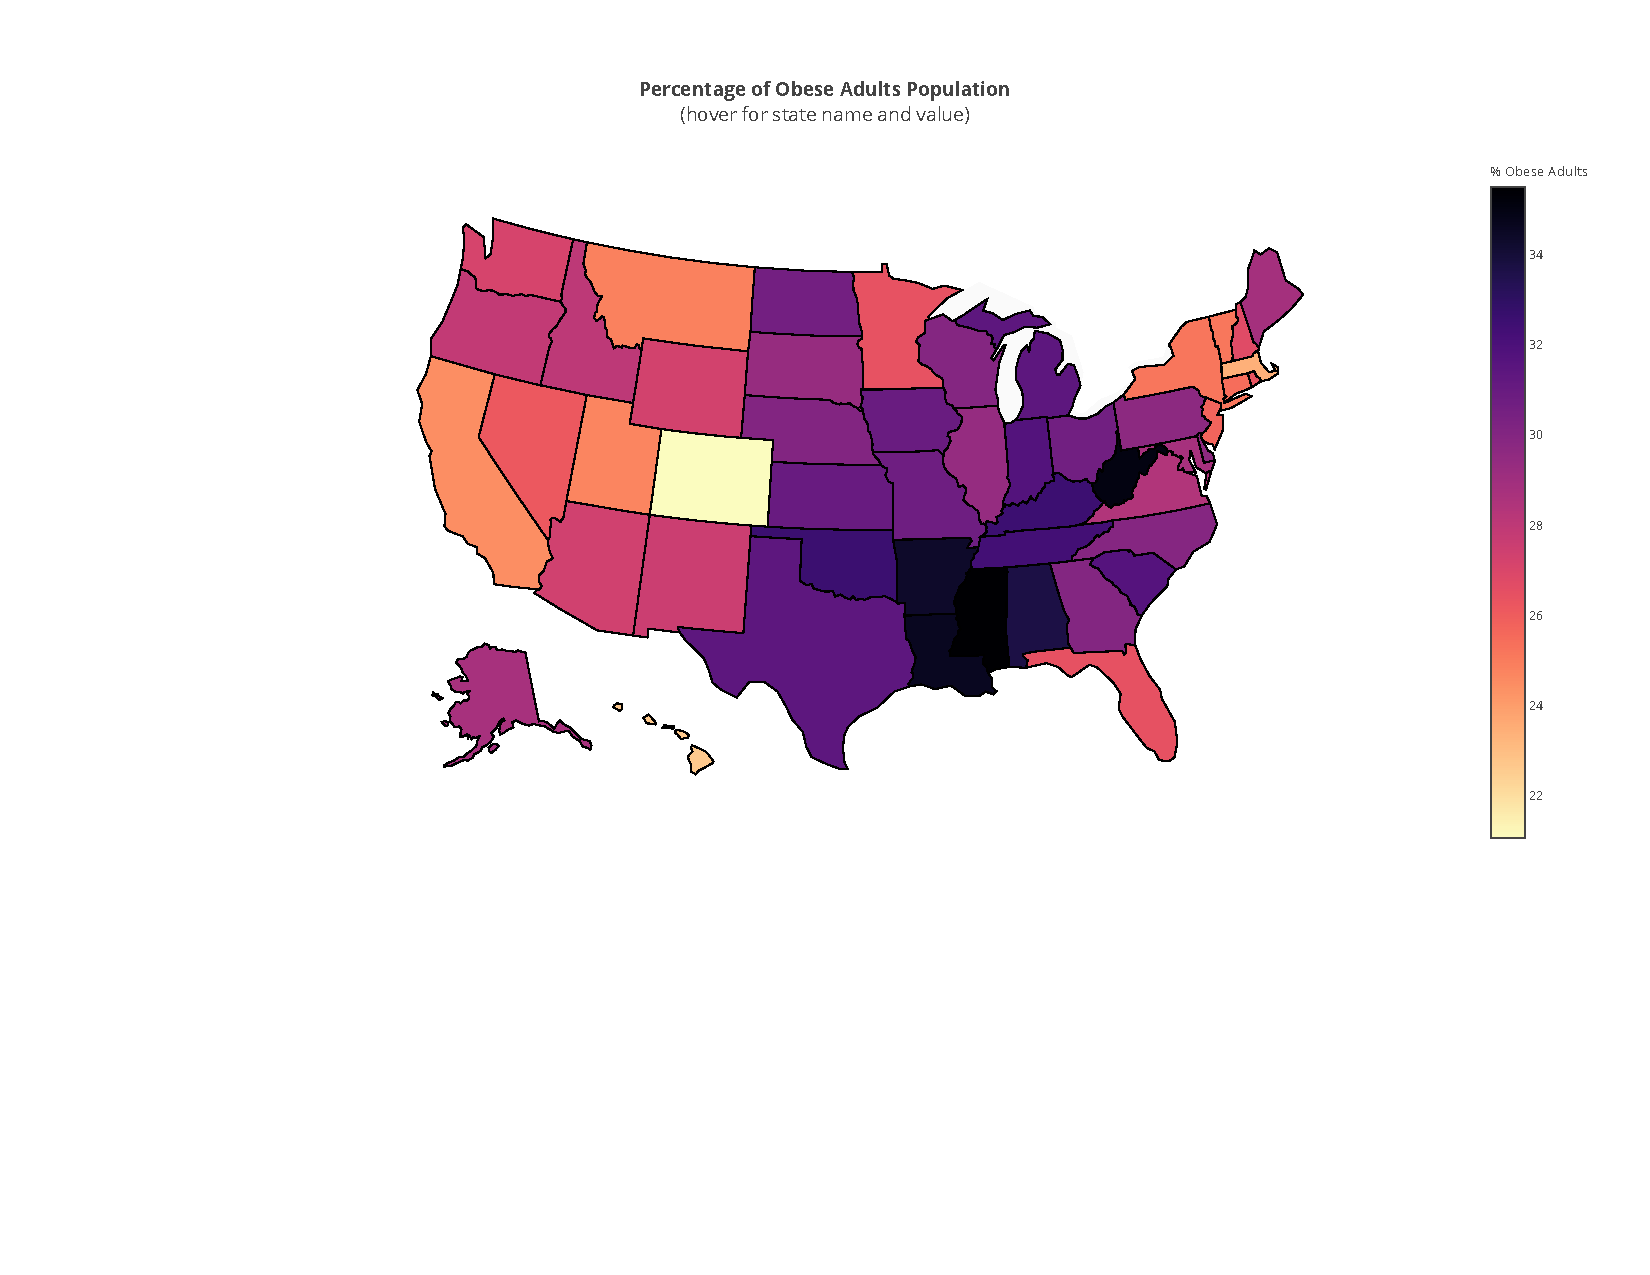
\includegraphics[width=\linewidth]{images/exploration_d3_map_obese_adults.pdf}
\label{fig:obesityByState}
\end{figure}
\begin{figure}[h]
\centering
\caption{}
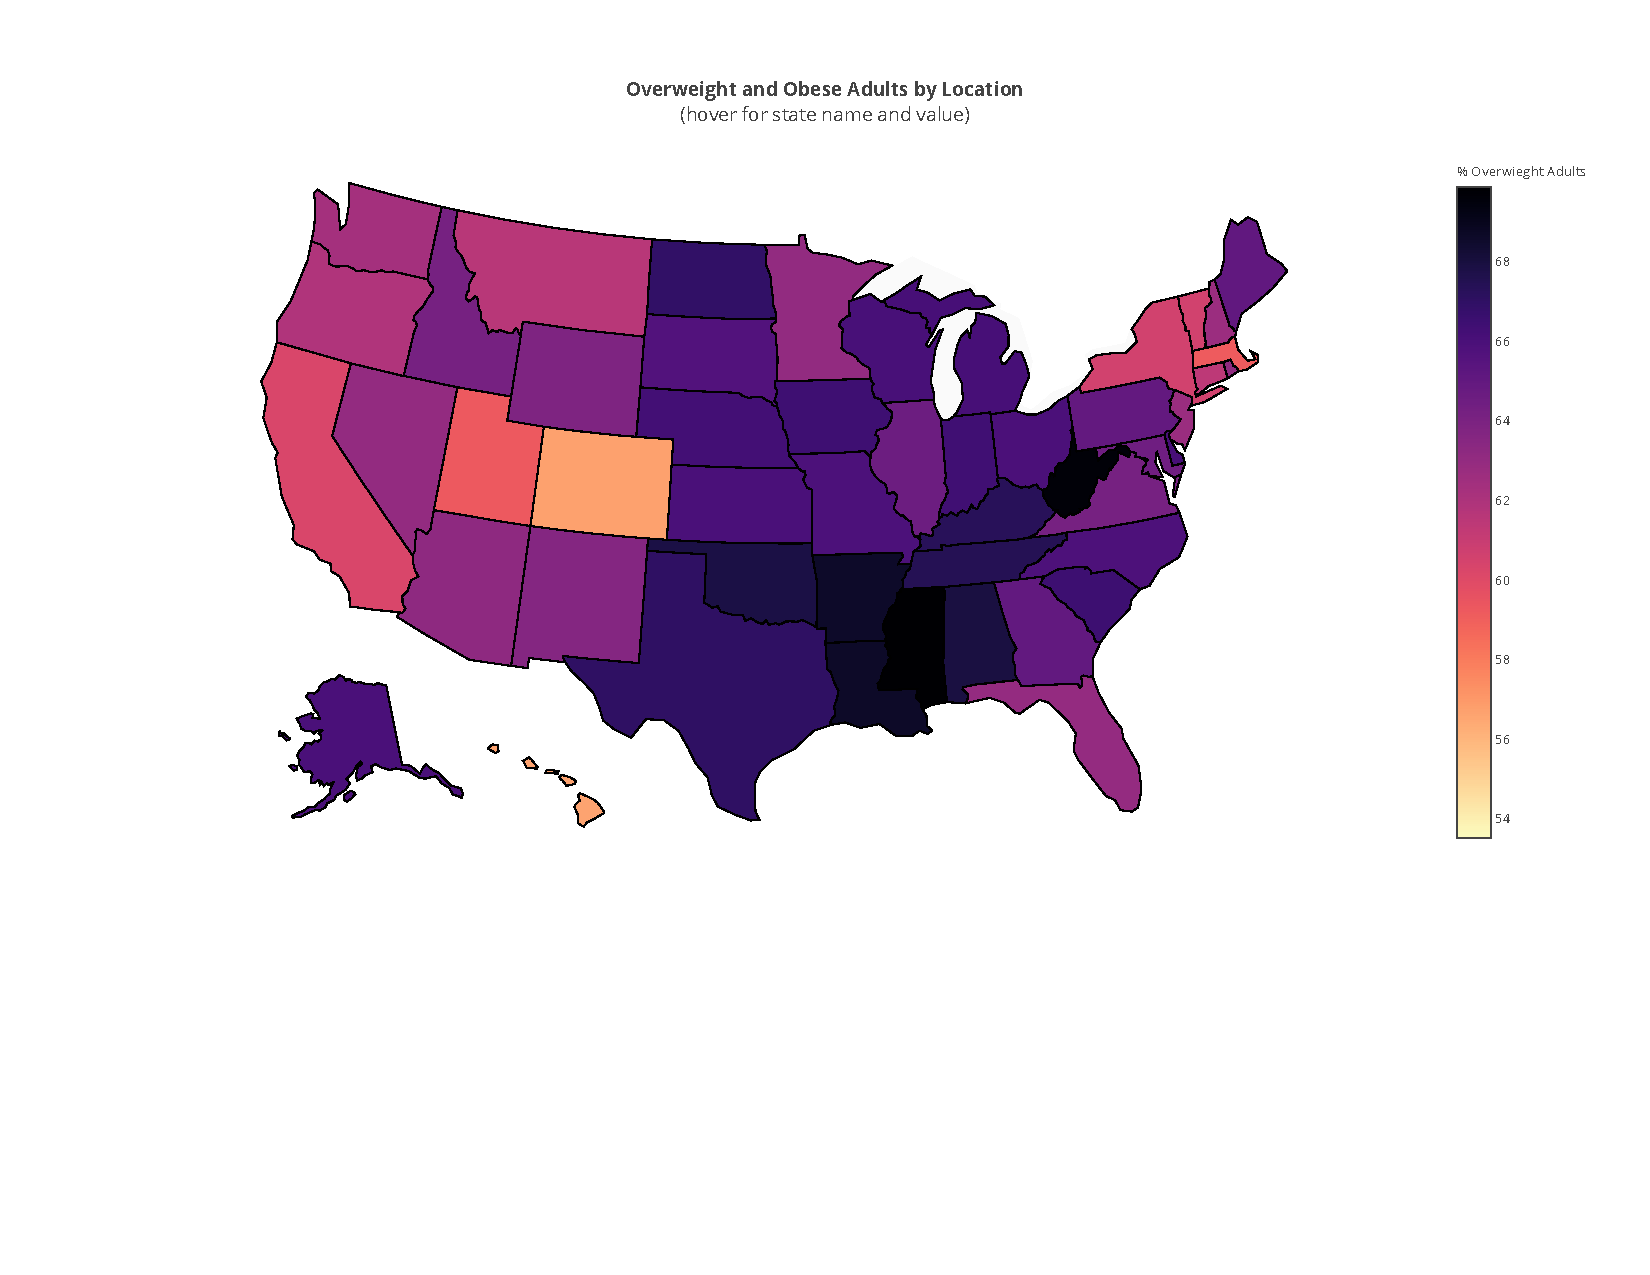
\includegraphics[width=\linewidth]{images/exploration_d3_map_overweight_adults.pdf}
\label{fig:overweightAdultsByLocation}
\end{figure}
\begin{figure}[h]
\centering
\caption{}
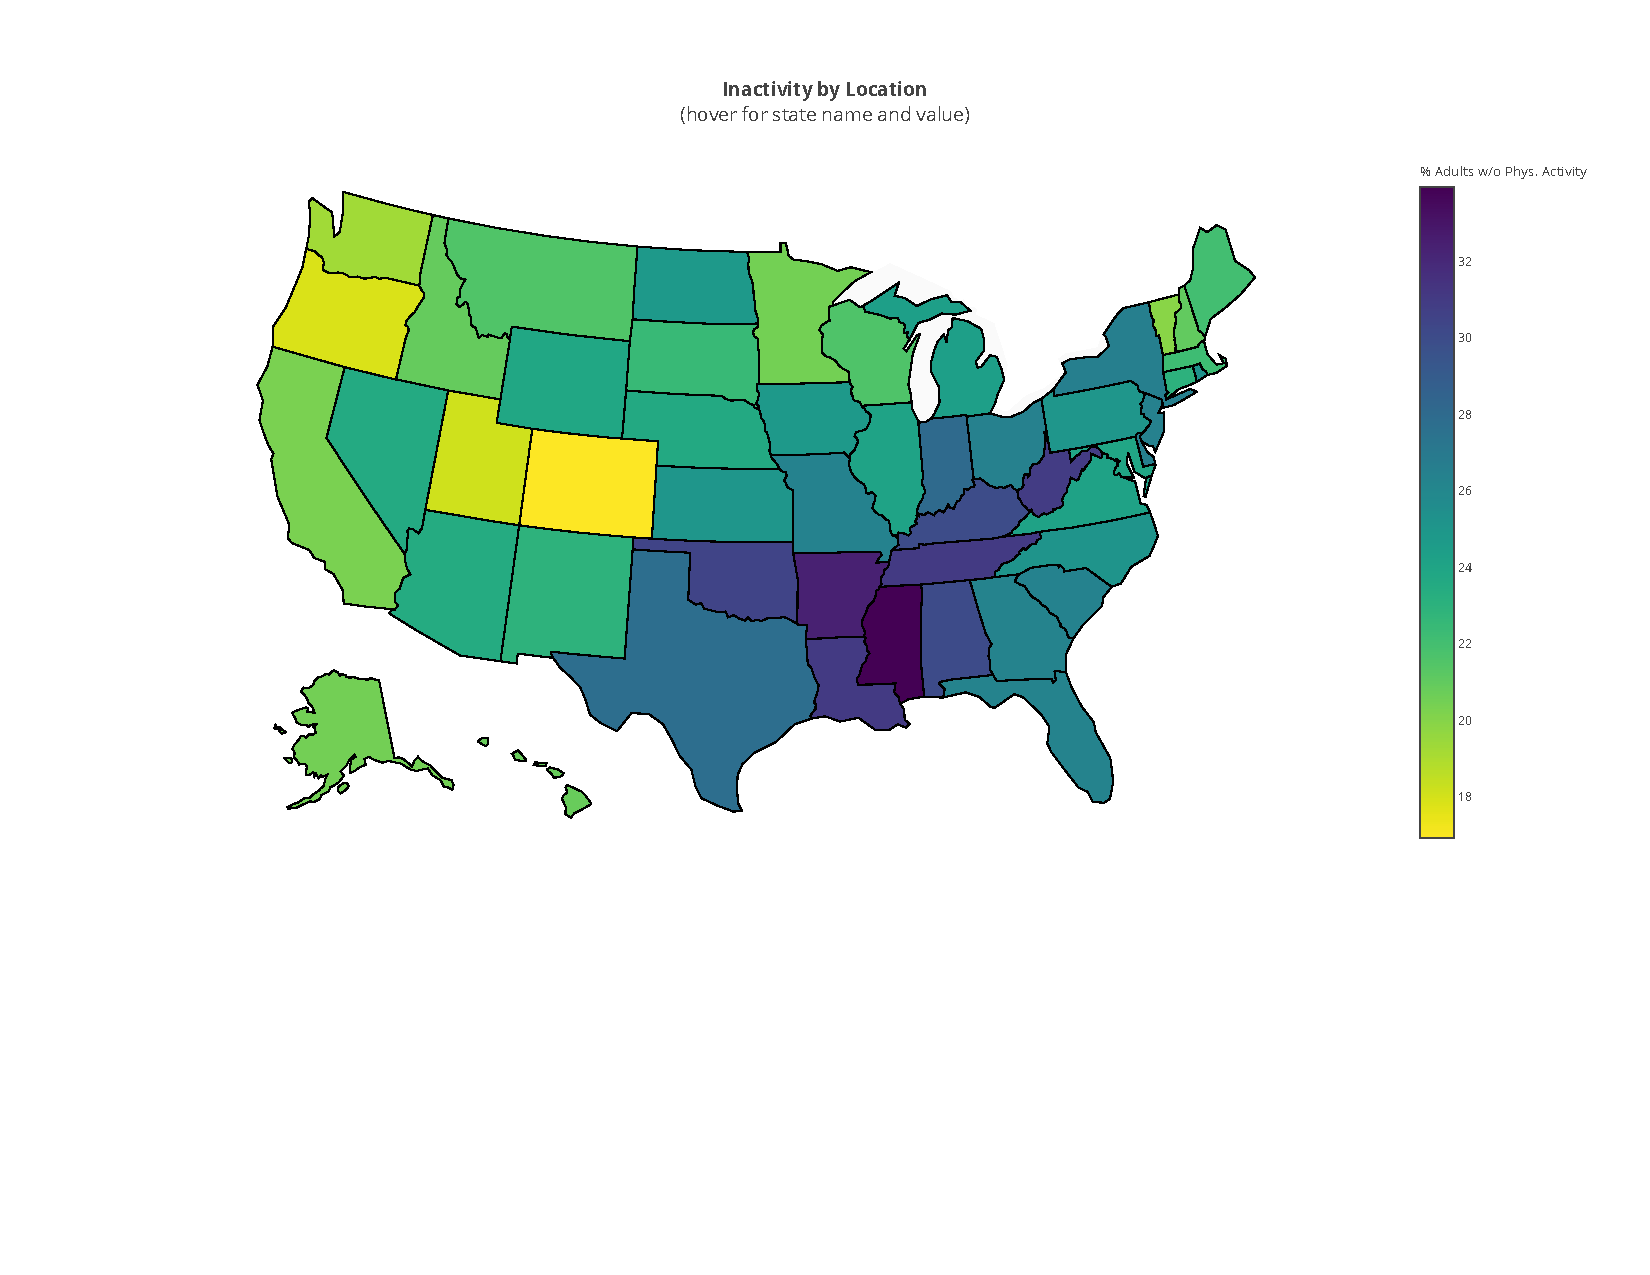
\includegraphics[width=\linewidth]{images/exploration_d3_map_inactive_adults.pdf}
\label{fig:inactivityByLocation}
\end{figure}
\begin{figure}[h]
\centering
\caption{}
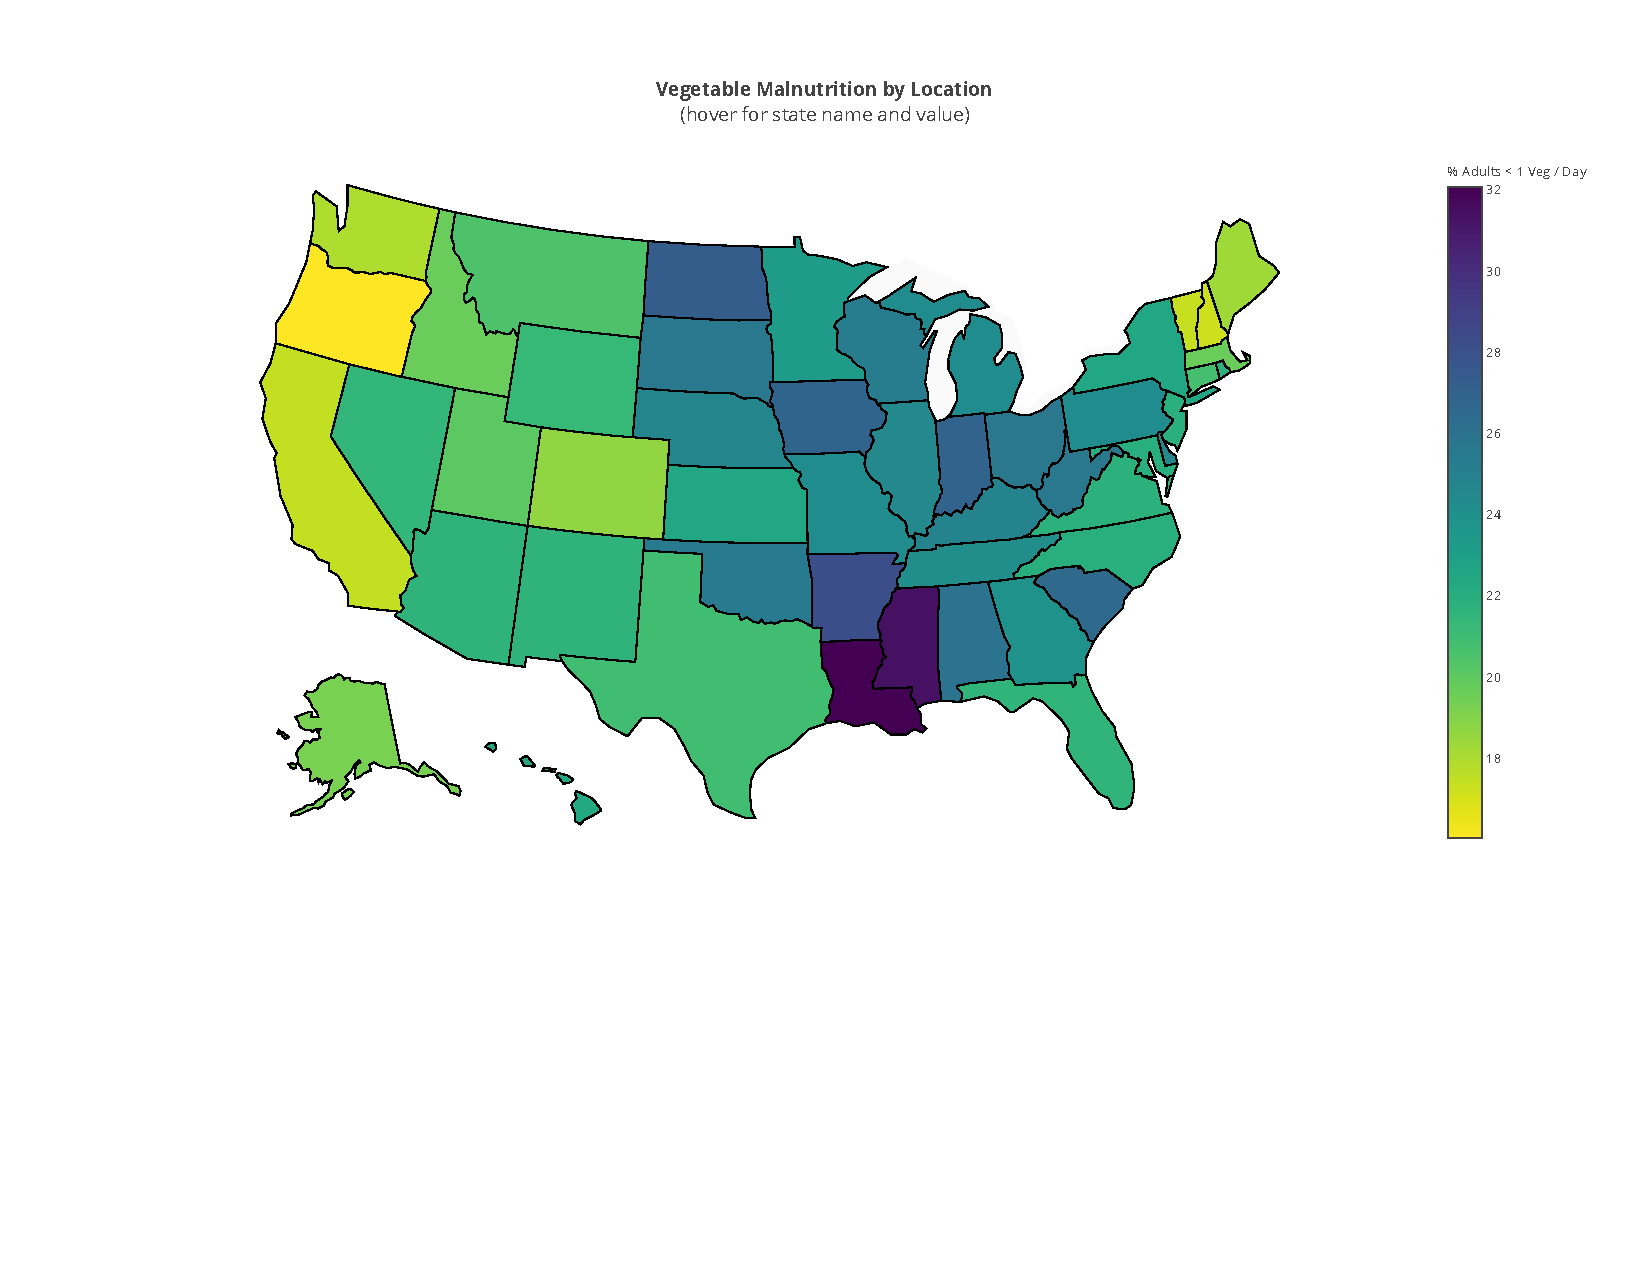
\includegraphics[width=\linewidth]{images/exploration_d3_map_veg_mal_adults.pdf}
\label{fig:vegetableMalnutritionByLocation}
\end{figure}
\begin{figure}[h]
\centering
\caption{}
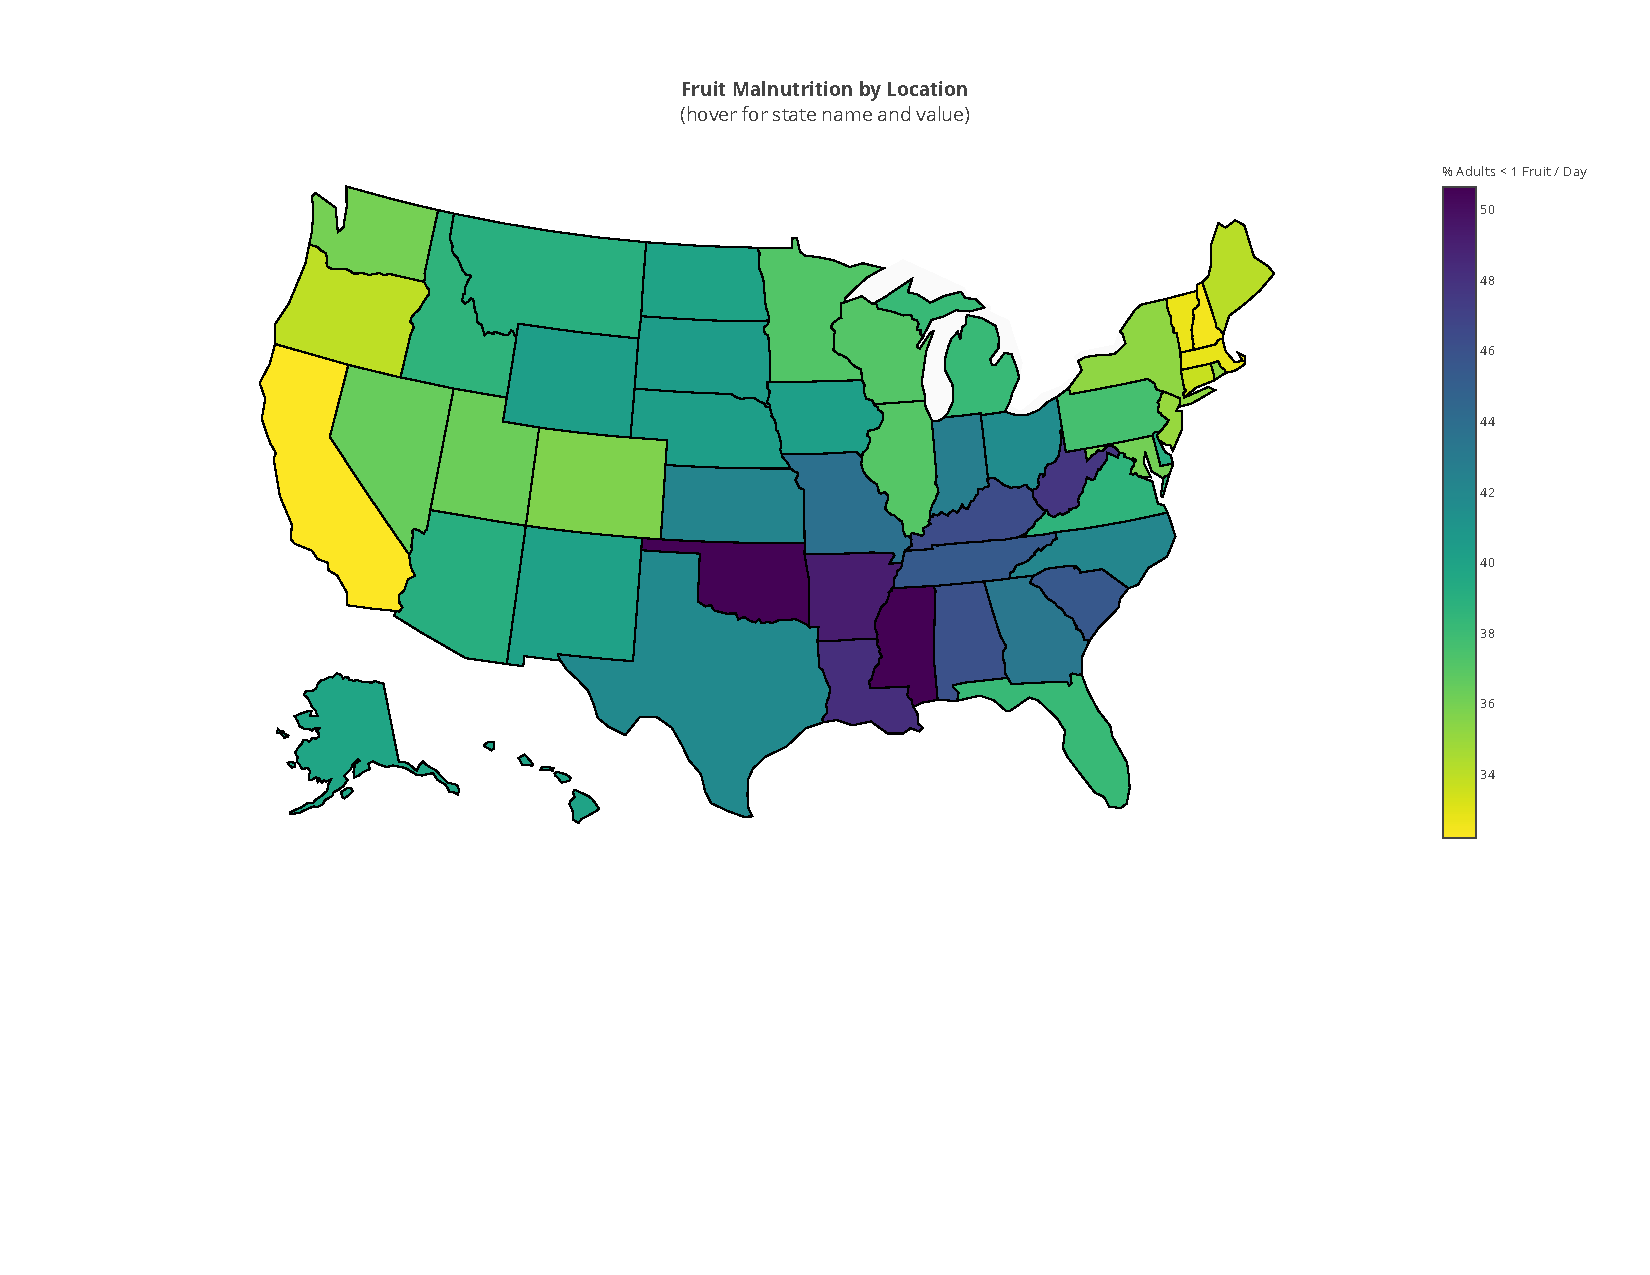
\includegraphics[width=\linewidth]{images/exploration_d3_map_fruit_mal_adults.pdf}
\label{fig:fruitMalnutritionByLocation}
\end{figure}
\\\\
From the exploratory analysis of making these plots, our team has identified several regional patterns, which will be important to understand when working on our clustering analysis, which was specified in the project proposal.
% Expand on these here- what are the patterns we see in these plots
We also wanted to start visualizing relationships between specific features to understand the dataset in finer detail. One way we did this was to look at the relationship between some of the other conditions and obesity on a state-by-state basis. These plots are shown in \cref{fig:fruitMalnutritionVsObesity,fig:aerobicActivityVsObesity,fig:noPhyActivityVsObesity}. 
\\\\
We also wanted to create plots to visually look at the percentages of adults in these other conditions and obesity based on age and educational risk factors. We have included a few of these plots in \cref{fig:aerobicVsMalnutrition,fig:trainingVsObesity,fig:vegMalnutritionVsObesity} below.
\begin{figure}[h]
\centering
\caption{Correlation between Mean (over Years) Vigerous Aerobic Activity and Obesity}
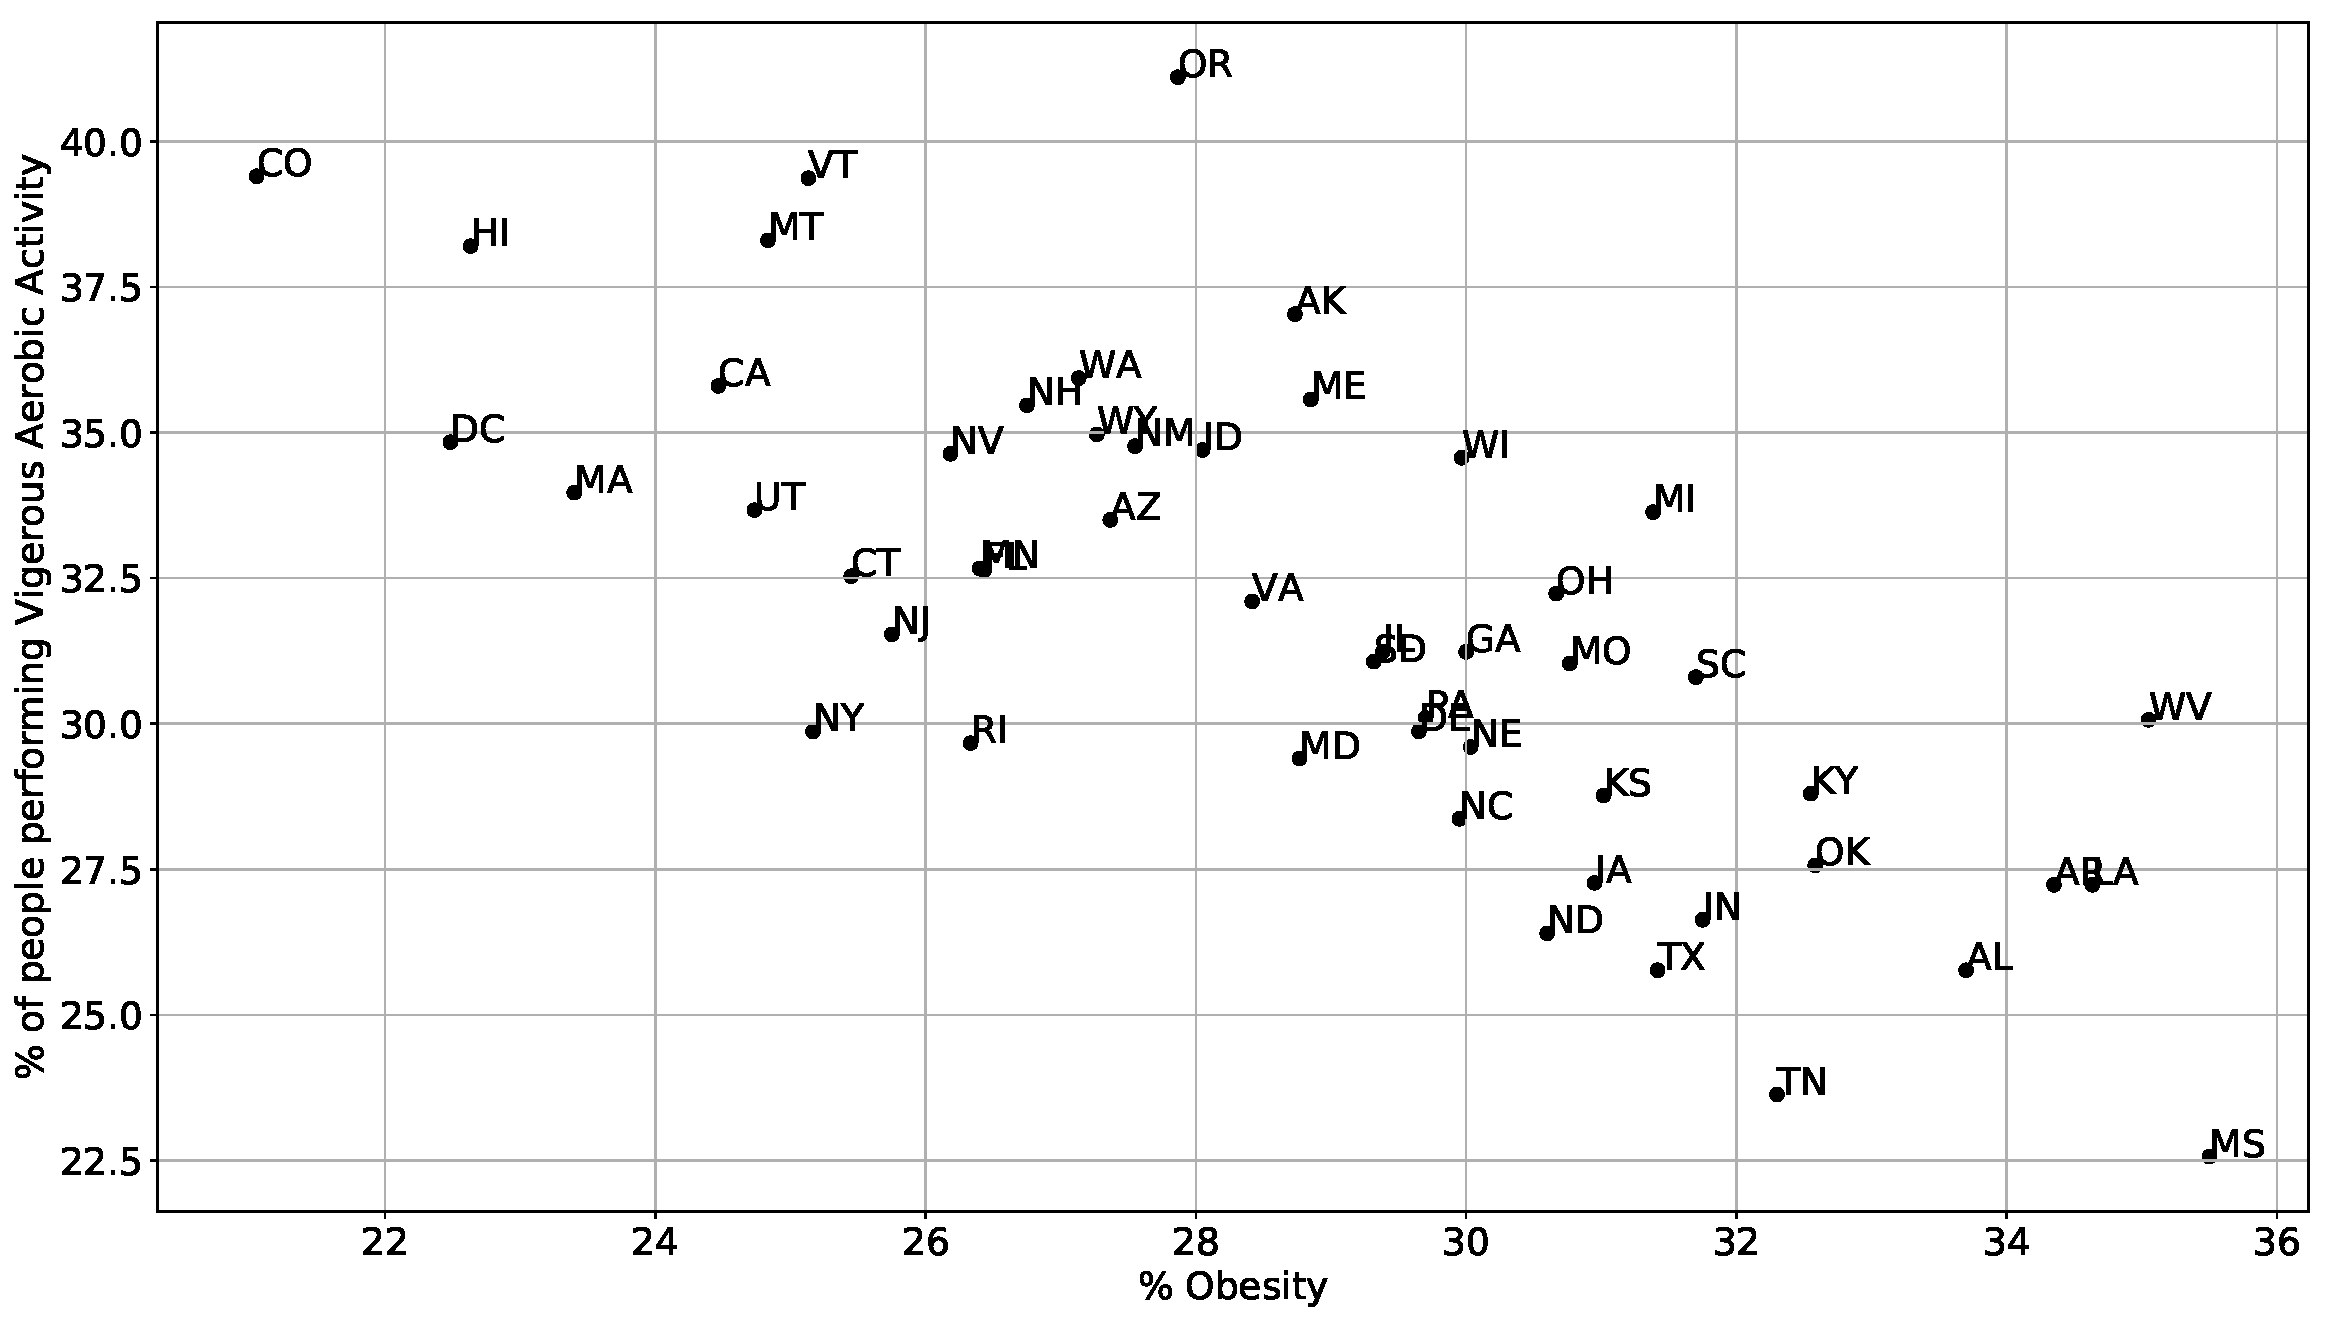
\includegraphics[width=\linewidth]{images/exploration_vigerous_aerobic_vs_obesity.pdf}
\label{fig:aerobicActivityVsObesity}
\end{figure}
\begin{figure}[h]
\centering
\caption{Correlation between Mean (over Years) Fruit Malnutrition and Obesity}
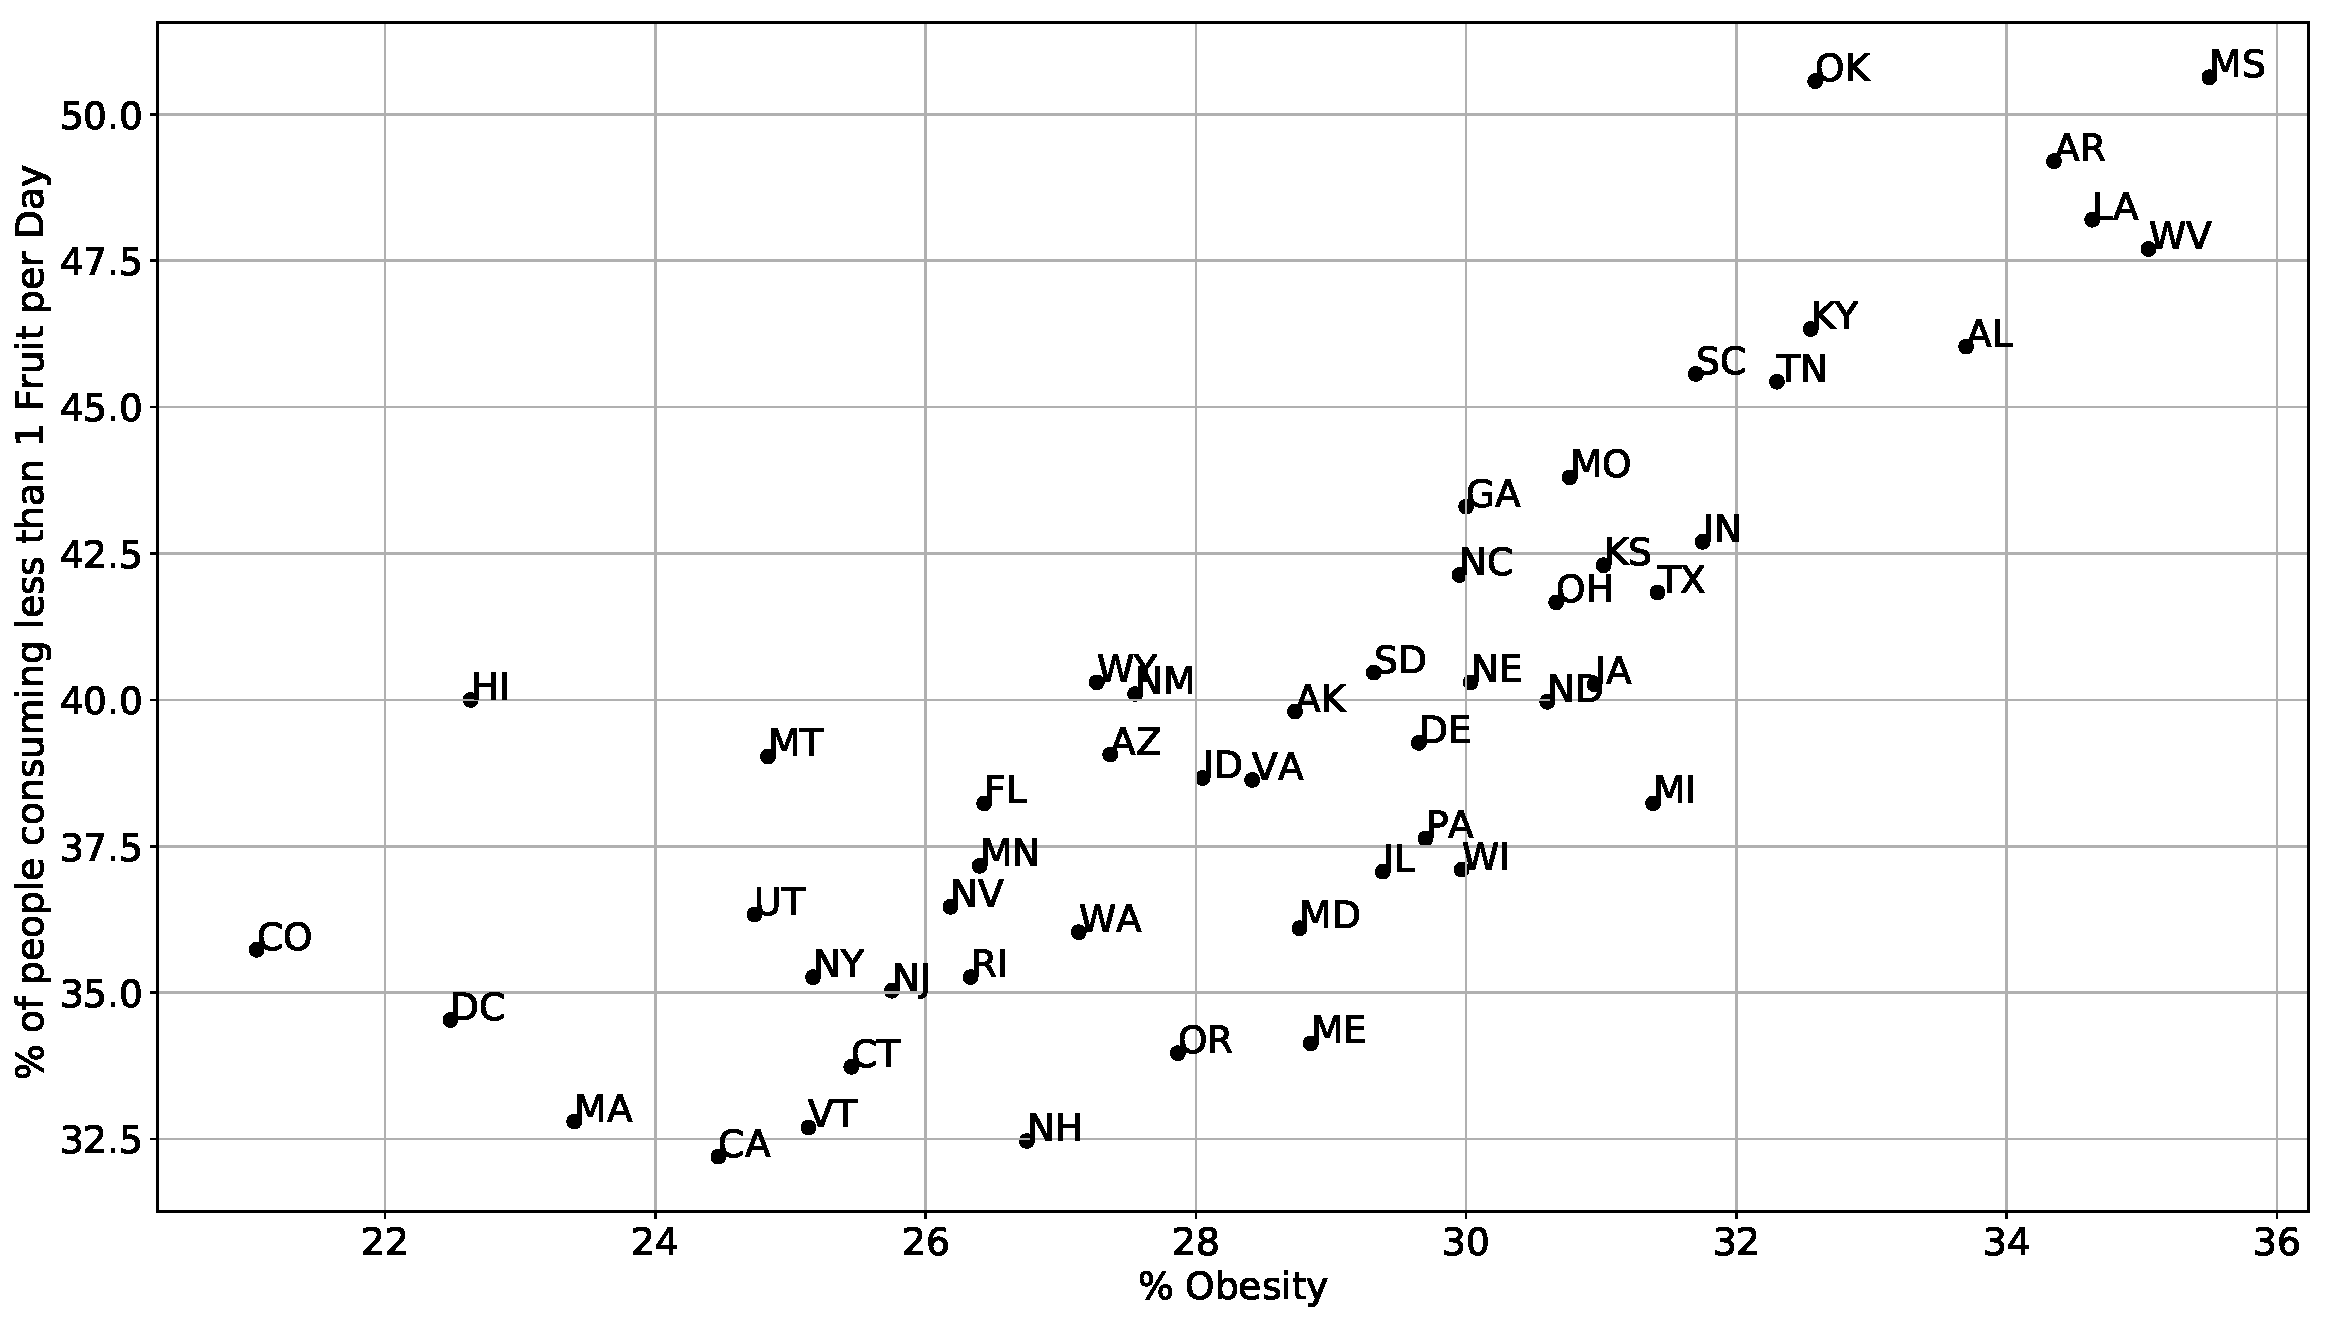
\includegraphics[width=\linewidth]{images/exploration_fruit_malnutrition_vs_obesity.pdf}
\label{fig:fruitMalnutritionVsObesity}
\end{figure}
% Explain specifically how they are made and what is plotted where, what error bars mean
% For scatters, this is a relation, but remember correlation doesn't imply causation, so don't claim that bad diet causes obesity, etc.
% For bar plots, this is just a visual representation for comparison
% Explain why they are useful- how they will drive next steps- what they allow us to understand

\section{Data Mining Analysis}
\label{dataanalysis}
In our data analysis, we were interested in clustering the CDC health behavior outcomes data we explored previously to investigate regional health outcomes and trends. We also collected data on socioeconomic risk factors (education status, race, and income) from Wikipedia \cite{demodata, eduratesdata, incomedata}, which was clustered separately and compared to the health behavior outcomes clusterings. 
We were interested in looking at similarities between these two sets of clusterings.
\\\\
To do this, we performed $k$-means, DBSCAN, and hierarchical clustering across these two datasets (CDC health behavior outcomes and the socioeconomic risk factors we put together from several articles on Wikipedia).

\subsection{Socioeconomic Risk Factors}
Before clustering, we first normalized the risk factor data to be scaled from $0$ to $1$. The specific features utilized were: percentage of residents who are high school graduates, percentage of residents with a Bachelor's degree, percentage of residents with an advanced degree, percentage of residents who are white, percentage of residents who are black or African American, percentage of residents who are American Indian or Alaska Native, percentage of residents who are Asian, percentage of residents who are Native Hawaiian or Other Pacific Islander, percentage of residents who are some other race, percentage of residents who are two or more races	, per capita income in dollars, median household income in dollars, and median family income in dollars.

\subsubsection{$k$-means}
To select a value of $k$, we performed $k$-means clustering for several values of $k$ and plotted the objectives as shown in \cref{fig:kmeanssocioselect}. From this plot, we identified $5$ as a value to use for clustering. We then performed $k$-means clustering with $k=5$ and plotted the results on a two-dimensional scatter plot (\cref{fig:kmeanssocioscat}) and state map (\cref{fig:kmeanssociomap}). The data was reduced to two dimensions for plotting by applying principal component analysis (PCA) and selecting the first two principal components.

\begin{figure}[h]
\centering
\caption{Objective function results as a function of $k$ used to select a value of $k$ for $k$-means clustering of socioeconomic risk factor data.}
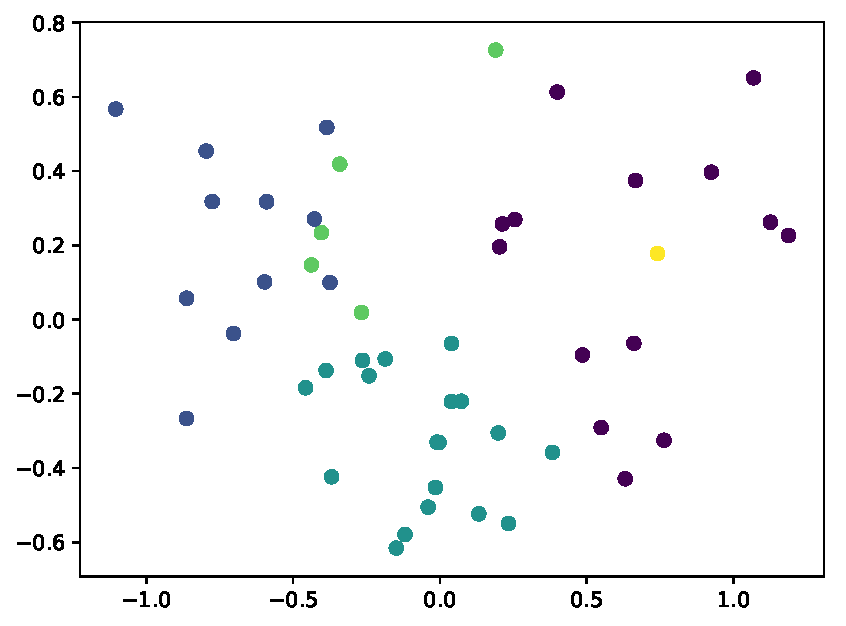
\includegraphics[width=\linewidth]{"images/socioeconomic_risk_factors_kmeans_2d_plot.pdf}
\label{fig:kmeanssocioselect}
\end{figure}

\begin{figure}[h]
\centering
\caption{Two dimensional plot of clusters from $k$-means clustering of socioeconomic risk factor data.}
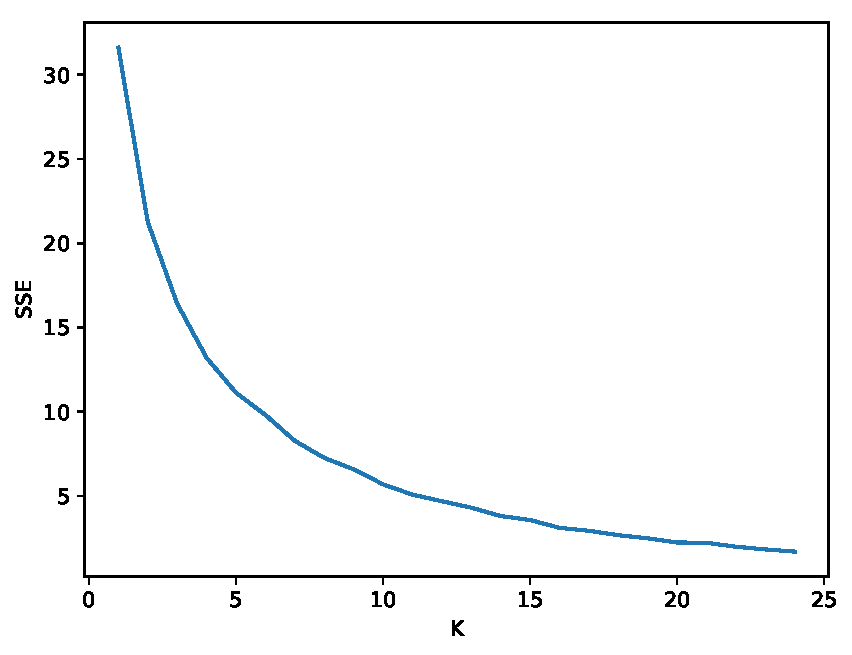
\includegraphics[width=\linewidth]{images/socioeconomic_risk_factors_kmeans_objc_tuning.pdf}
\label{fig:kmeanssocioscat}
\end{figure}

\begin{figure}[h]
\centering
\caption{Geographic plot of clusters from $k$-means clustering of socioeconomic risk factor data.}
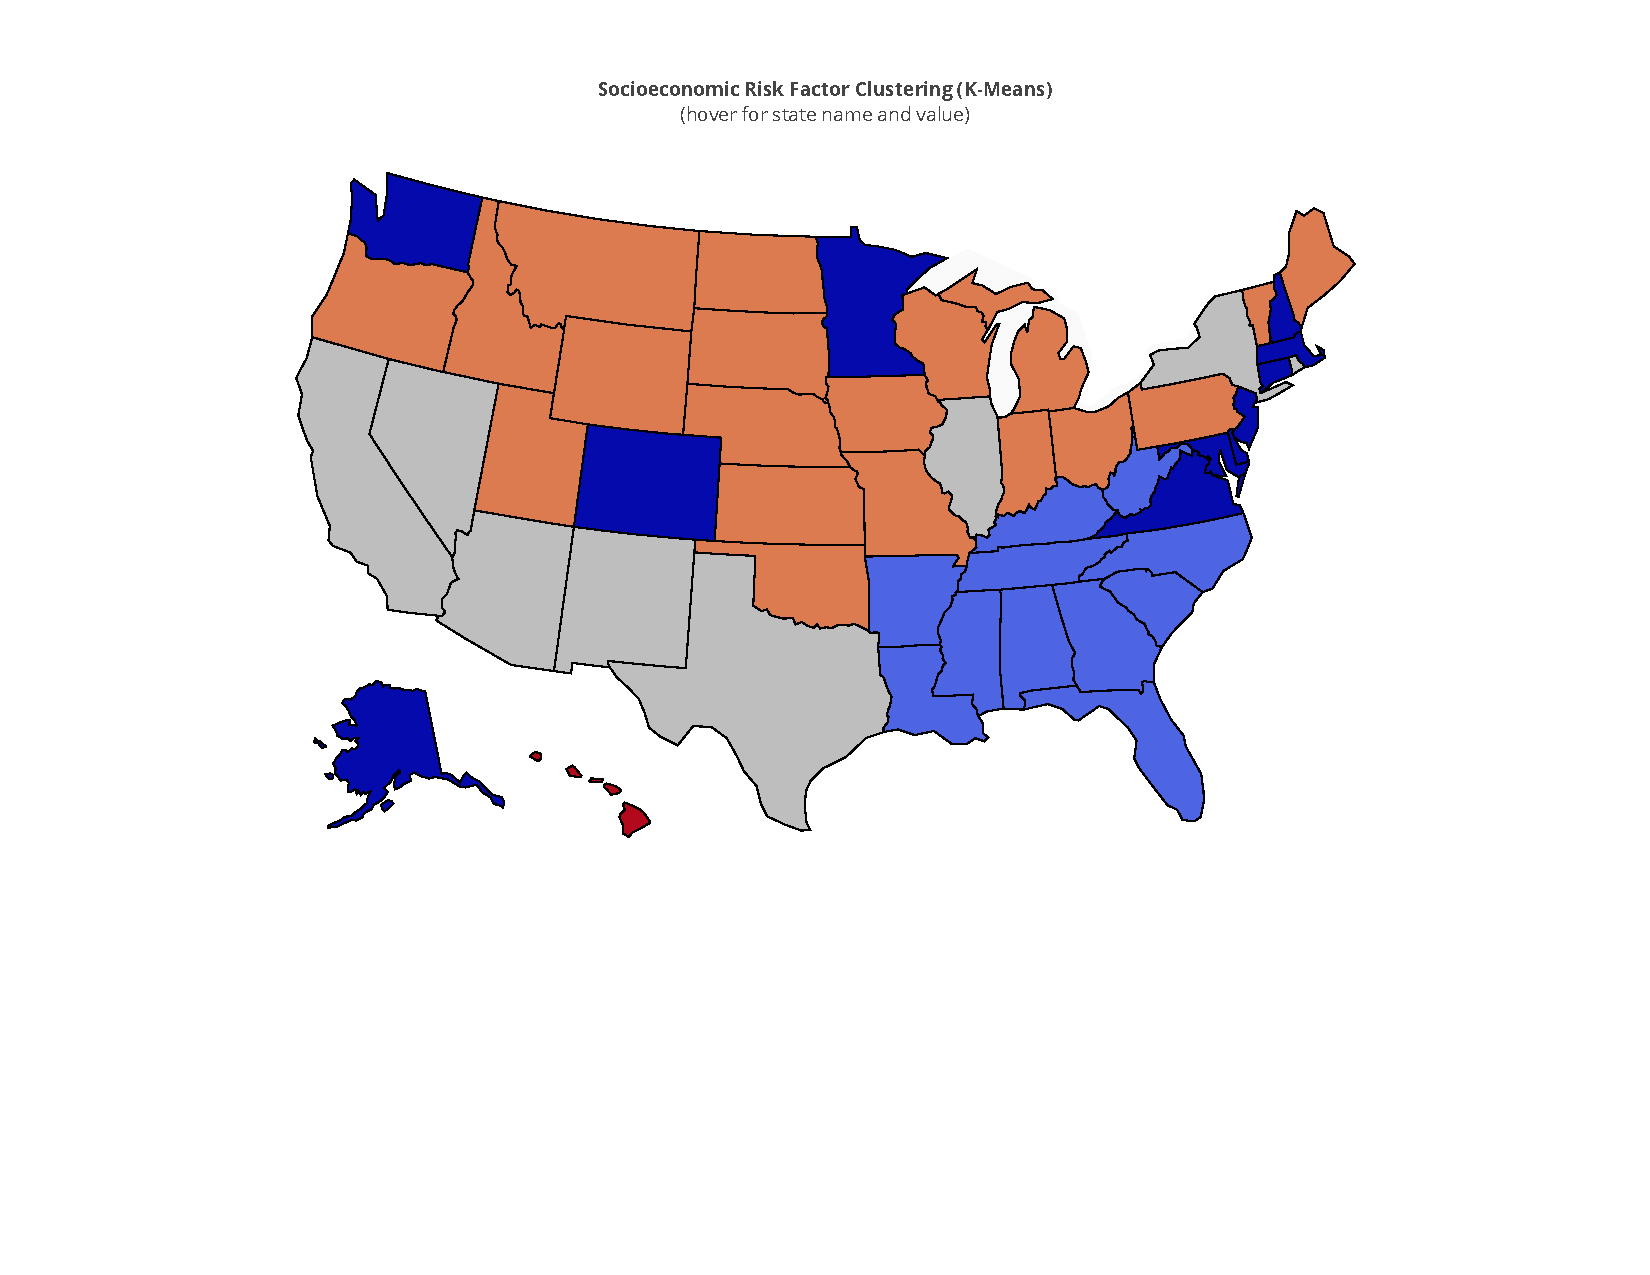
\includegraphics[width=\linewidth]{images/socioeconomic_risk_factor_kmeans_map.pdf}
\label{fig:kmeanssociomap}
\end{figure}

\subsubsection{DBSCAN}
We then performed DBSCAN with $\epsilon = 0.6$ and $minPts = 6$ because they achieved less than $5\%$ noise. This resulted in a single cluster with four noise points as seen in \cref{fig:dbsocioscat,fig:dbsociomap}. Like performed previously, the data was reduced to two dimensions for plotting by applying principal component analysis (PCA) and selecting the first two principal components.

\begin{figure}[h]
\centering
\caption{Two dimensional plot of clusters from DBSCAN clustering of socioeconomic risk factor data.}
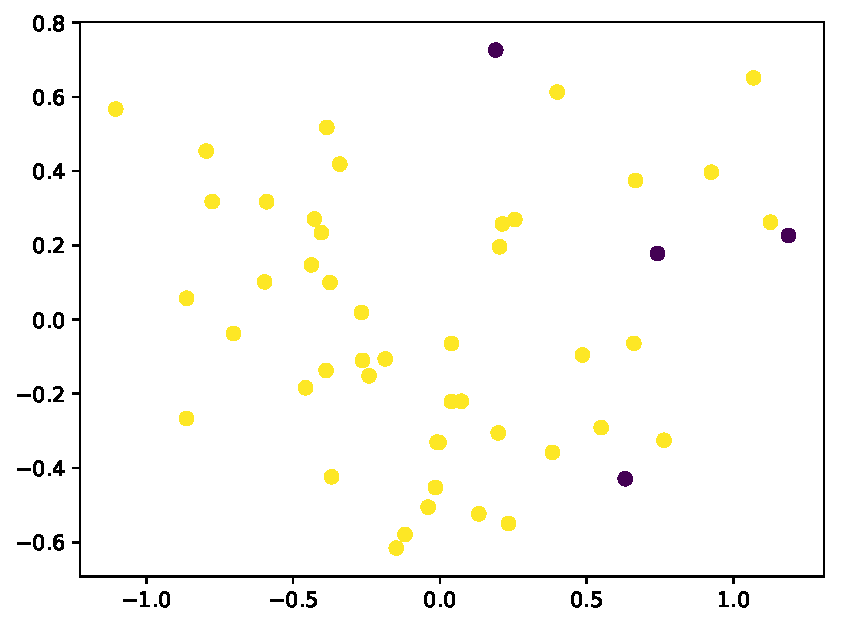
\includegraphics[width=\linewidth]{images/socioeconomic_risk_factors_dbscan_2d_plot.pdf}
\label{fig:dbsocioscat}
\end{figure}

\begin{figure}[h]
\centering
\caption{Geographic plot of clusters from DBSCAN clustering of socioeconomic risk factor data.}
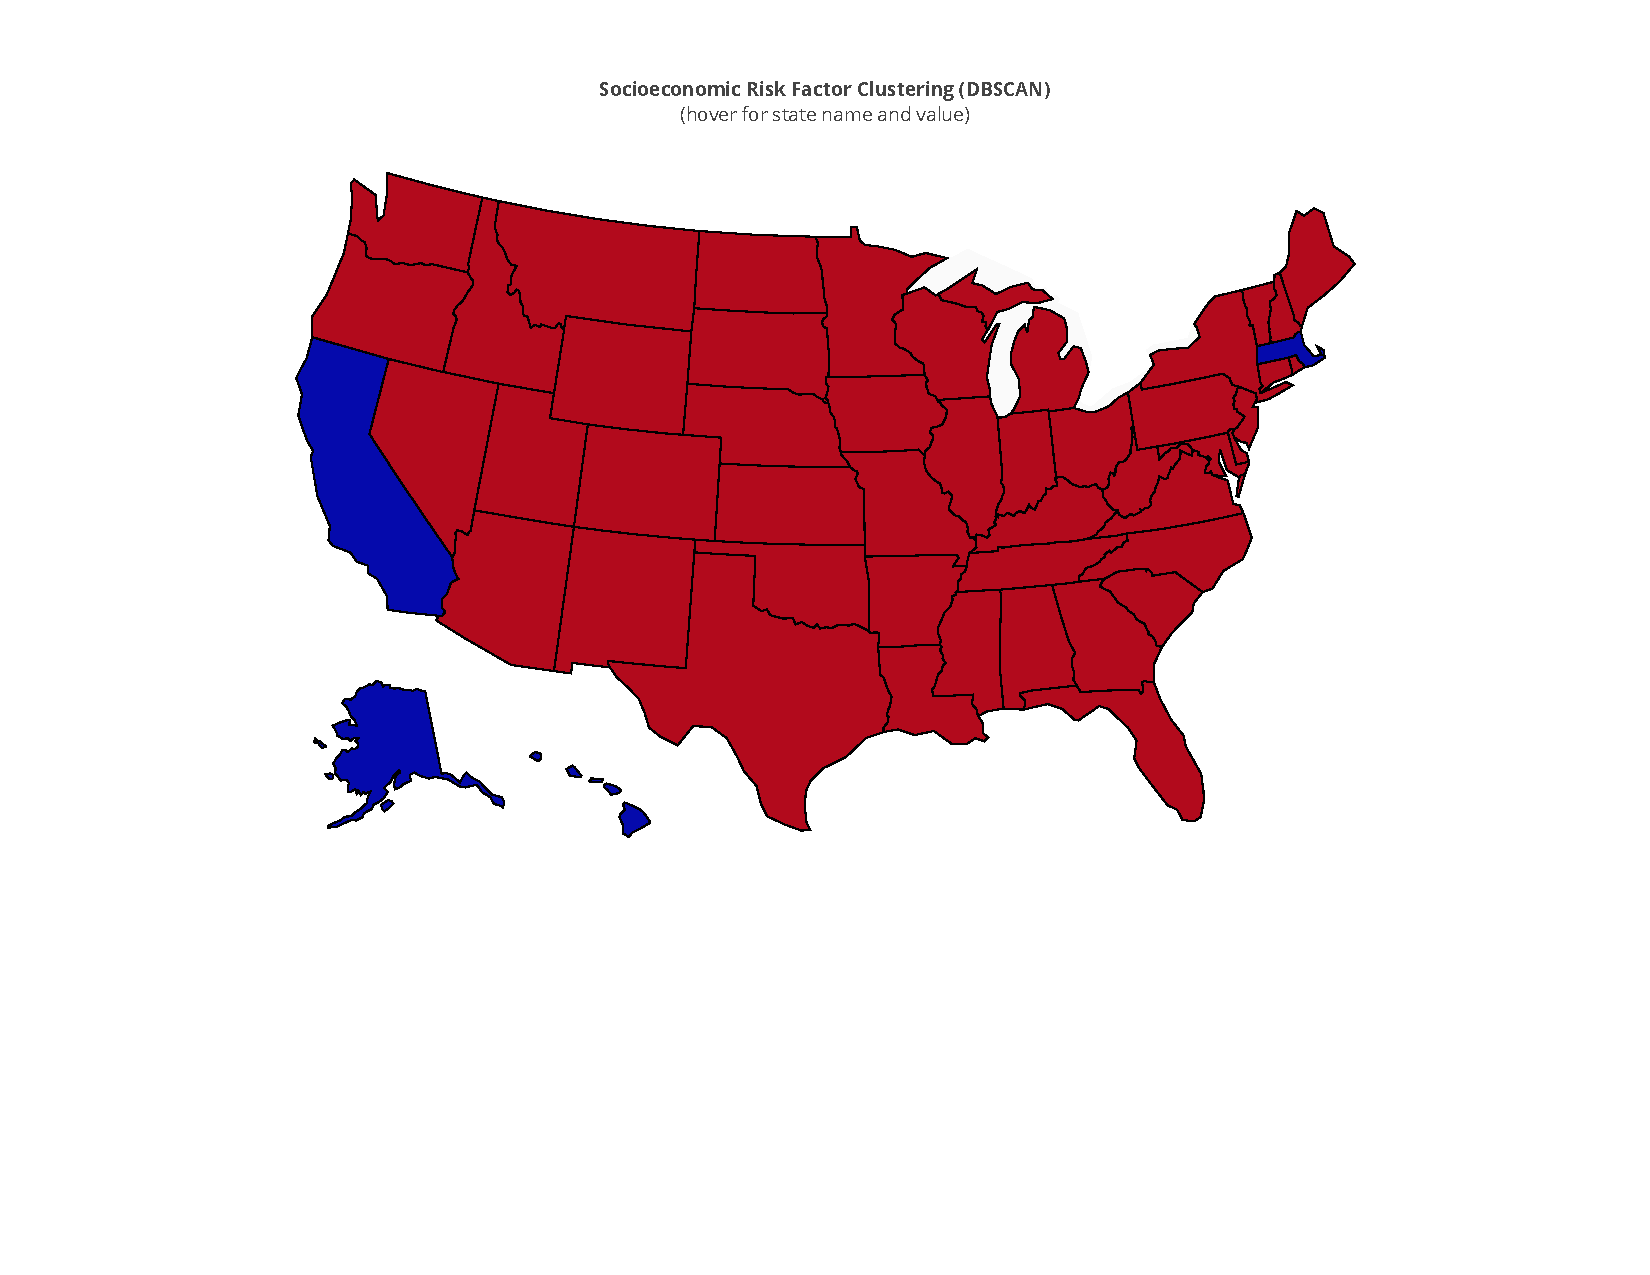
\includegraphics[width=\linewidth]{images/socioeconomic_risk_factor_dbscan_map.pdf}
\label{fig:dbsociomap}
\end{figure}

\subsubsection{Hierarchical Clustering}
We then performed agglomerative hierarchical clustering using a Ward distance metric. The Ward metric was selected after comparing results from the single, complete, and average linkage metrics. This clustering is shown in \cref{fig:dbsociodg}.

\begin{figure}[h]
\centering
\caption{}
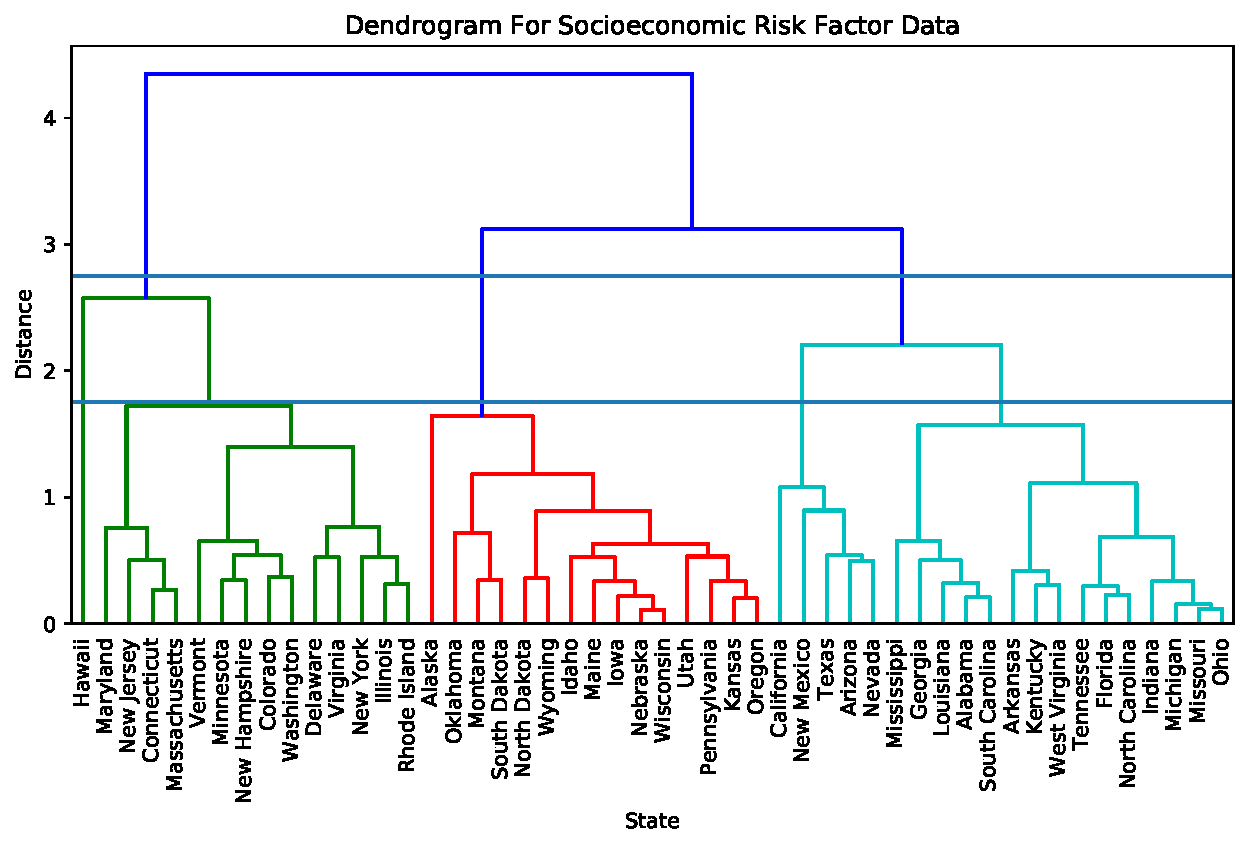
\includegraphics[width=\linewidth]{images/socioeconomic_risk_factors_agglomerative_dendrogram.pdf}
\label{fig:dbsociodg}
\end{figure}

\subsection{CDC Health Behavior and Outcomes}
Before clustering, we first normalized the CDC health behavior and outcomes data to be scaled from $0$ to $1$. The specific features utilized were: percentage of residents who are obese, percentage of residents who are overweight, percentage of residents who do not engage in physical activity, percentage of residents who engage in vigerous aerobic activity, percentage of residents who consume less than one vegetable per day, and percentage of residents who consume less than one fruit per day.

\subsubsection{$k$-means}
To select a value of $k$, we performed $k$-means clustering for several values of $k$ and plotted the objectives as shown in \cref{fig:kmeanshealthselect}. From this plot, we identified $3$ as a value to use for clustering. We then performed $k$-means clustering with $k=3$ and plotted the results on a two-dimensional scatter plot (\ref{fig:kmeanshealthscat}) and state map (\ref{fig:kmeanshealthmap}). The data was reduced to two dimensions for plotting by applying principal component analysis (PCA) and selecting the first two principal components.

\begin{figure}[h]
\centering
\caption{Objective function results as a function of $k$ used to select a value of $k$ for $k$-means clustering of health behavior and outcome data.}
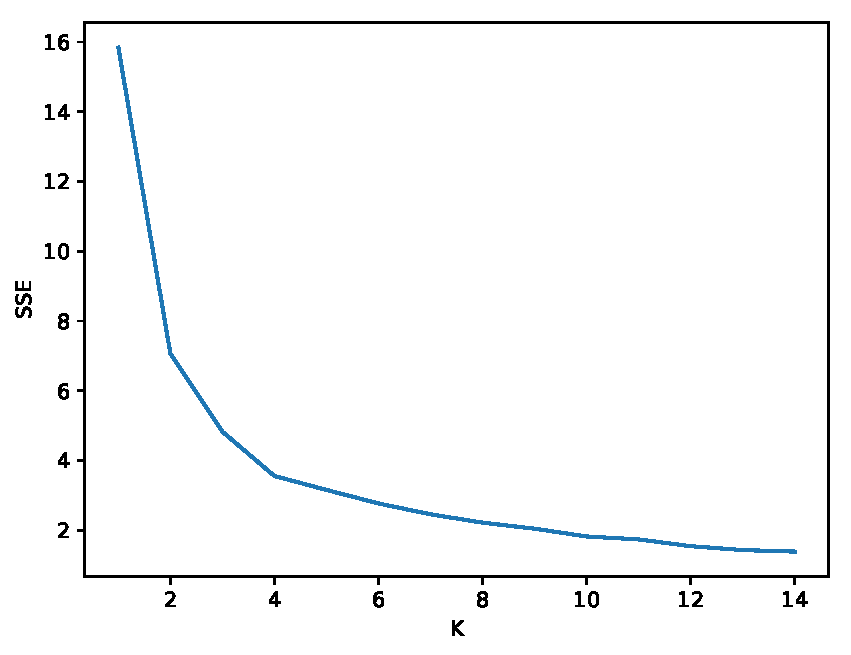
\includegraphics[width=\linewidth]{images/cdc_health_behavior_and_outcomes_kmeans_obj_tuning.pdf}
\label{fig:kmeanshealthselect}
\end{figure}

\begin{figure}[h]
\centering
\caption{Two dimensional plot of clusters from $k$-means clustering of health behavior and outcome data.}
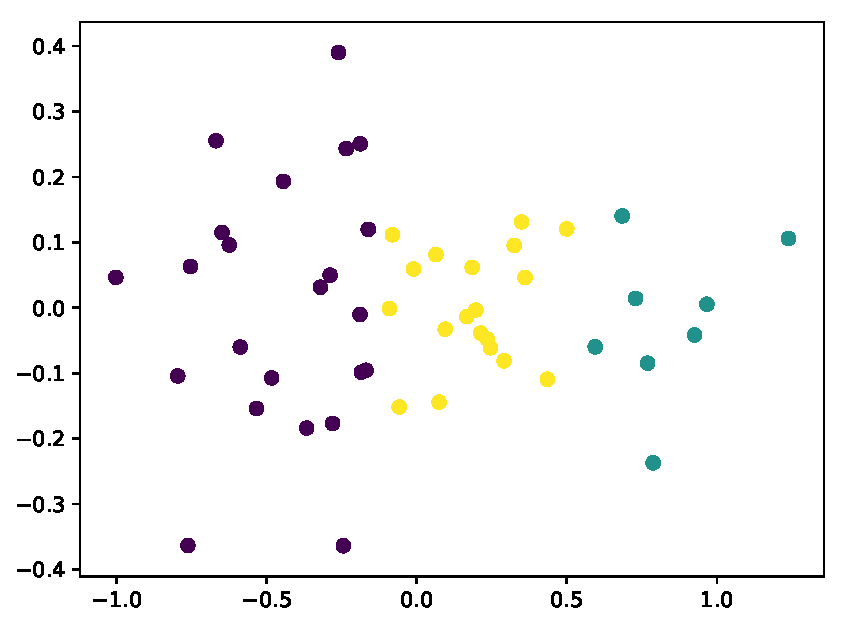
\includegraphics[width=\linewidth]{images/cdc_health_behavior_and_outcomes_kmeans_2d_plot.pdf}
\label{fig:kmeanshealthscat}
\end{figure}

\begin{figure}[h]
\centering
\caption{Geographic plot of clusters from $k$-means clustering of health behavior and outcome data.}
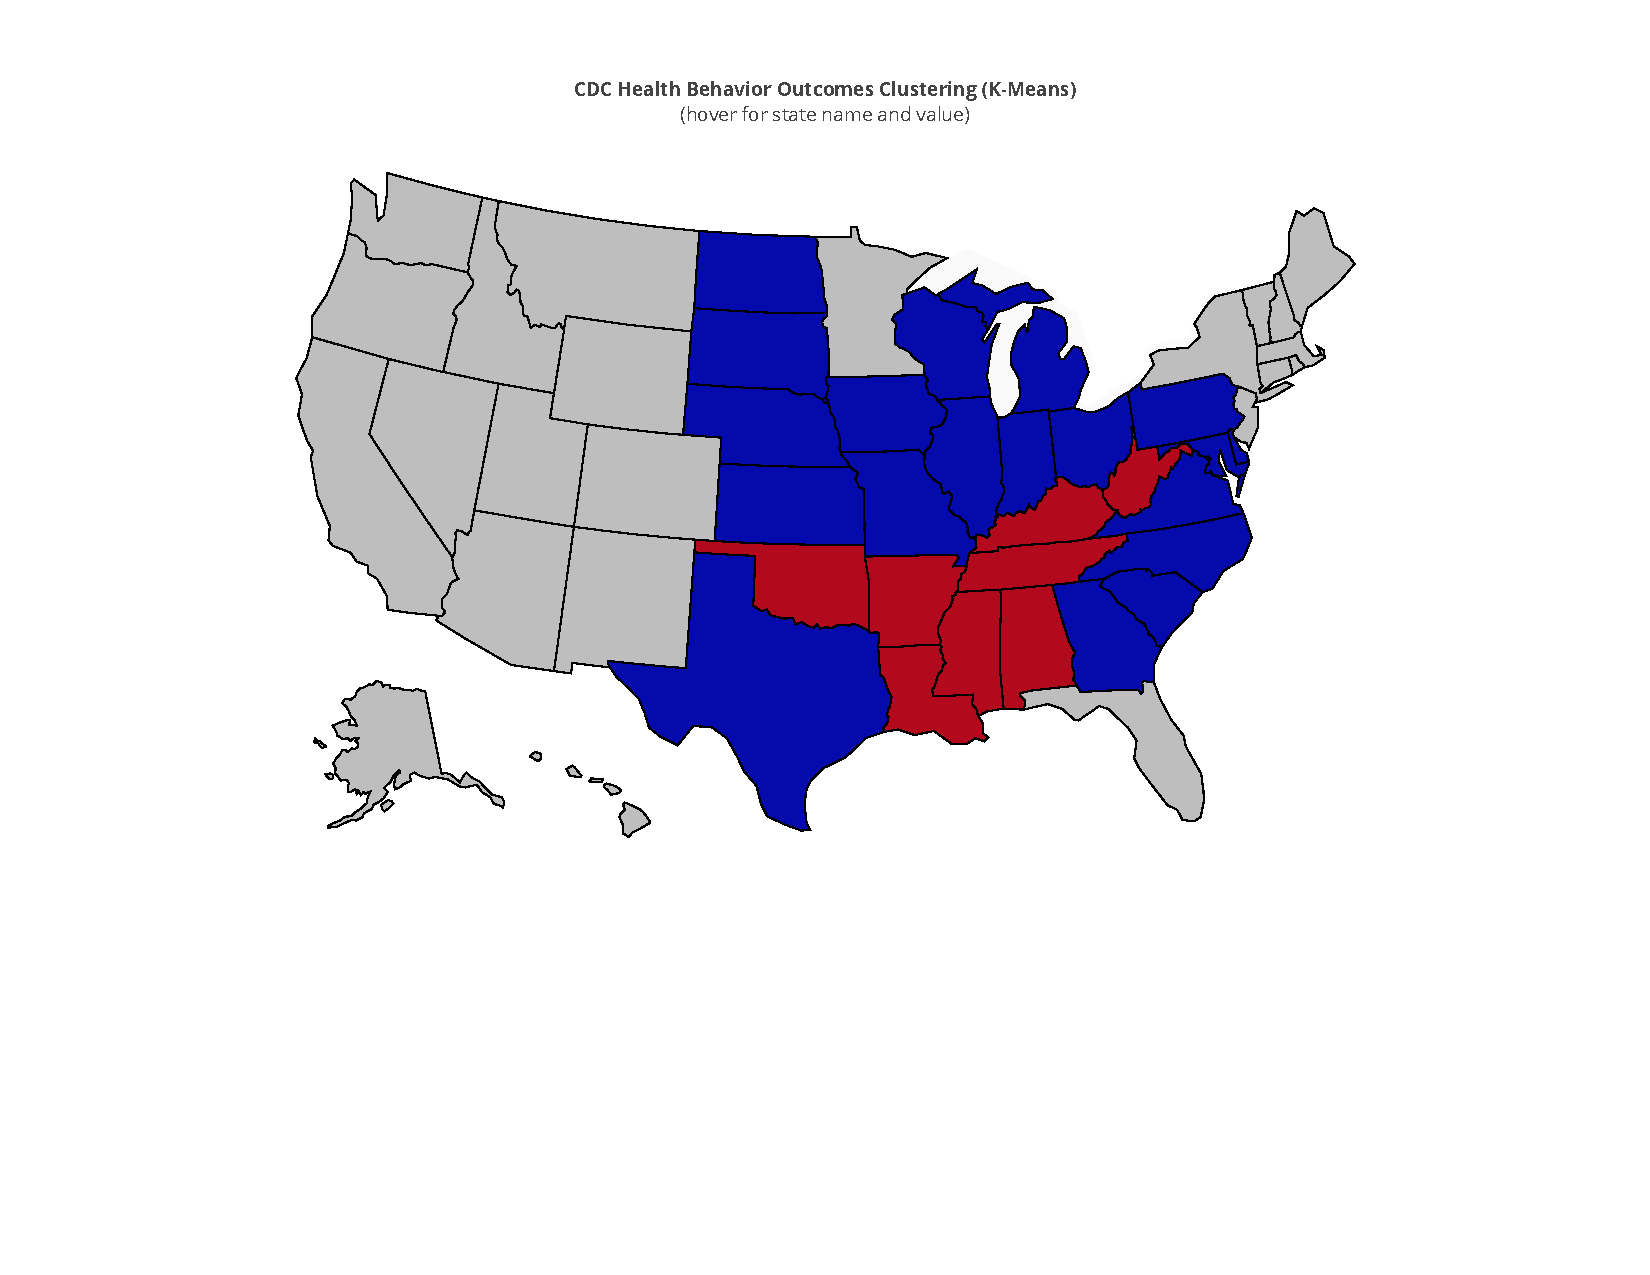
\includegraphics[width=\linewidth]{images/cdc_health_behavior_and_outcomes_kmeans_map.pdf}
\label{fig:kmeanshealthmap}
\end{figure}

\subsubsection{DBSCAN}
We then performed DBSCAN with $\epsilon = 0.2$ and $minPts = 3$ because they achieved less than $5\%$ noise. This resulted in a single cluster with four noise points as seen in \cref{fig:dbhealthscat,fig:dbhealthmap}. Like performed previously, the data was reduced to two dimensions for plotting by applying principal component analysis (PCA) and selecting the first two principal components.

\begin{figure}[h]
\centering
\caption{Two dimensional plot of clusters from DBSCAN clustering of health behavior and outcome data.}
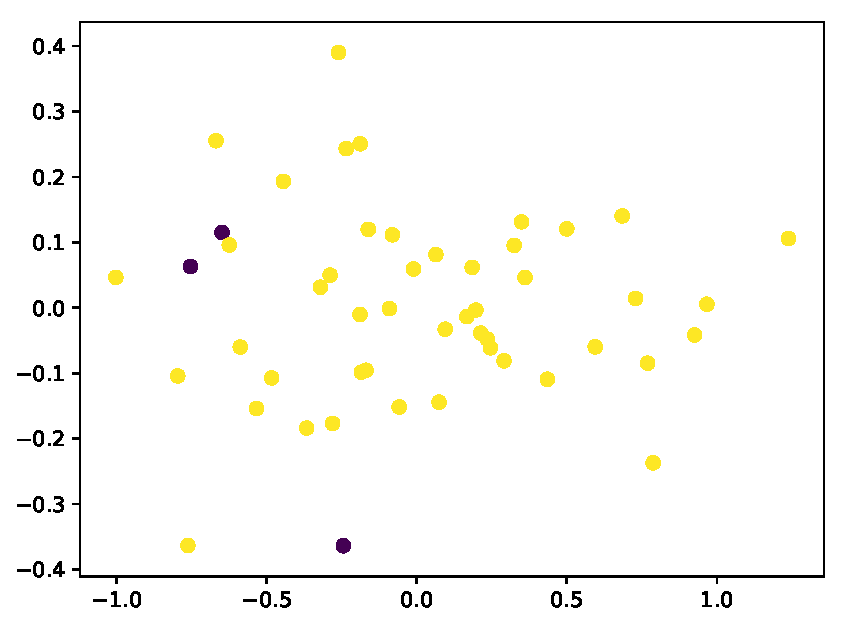
\includegraphics[width=\linewidth]{images/cdc_health_behavior_and_outcomes_dbscan_2d_plot.pdf}
\label{fig:dbhealthscat}
\end{figure}

\begin{figure}[h]
\centering
\caption{Geographic plot of clusters from DBSCAN clustering of health behavior and outcome data.}
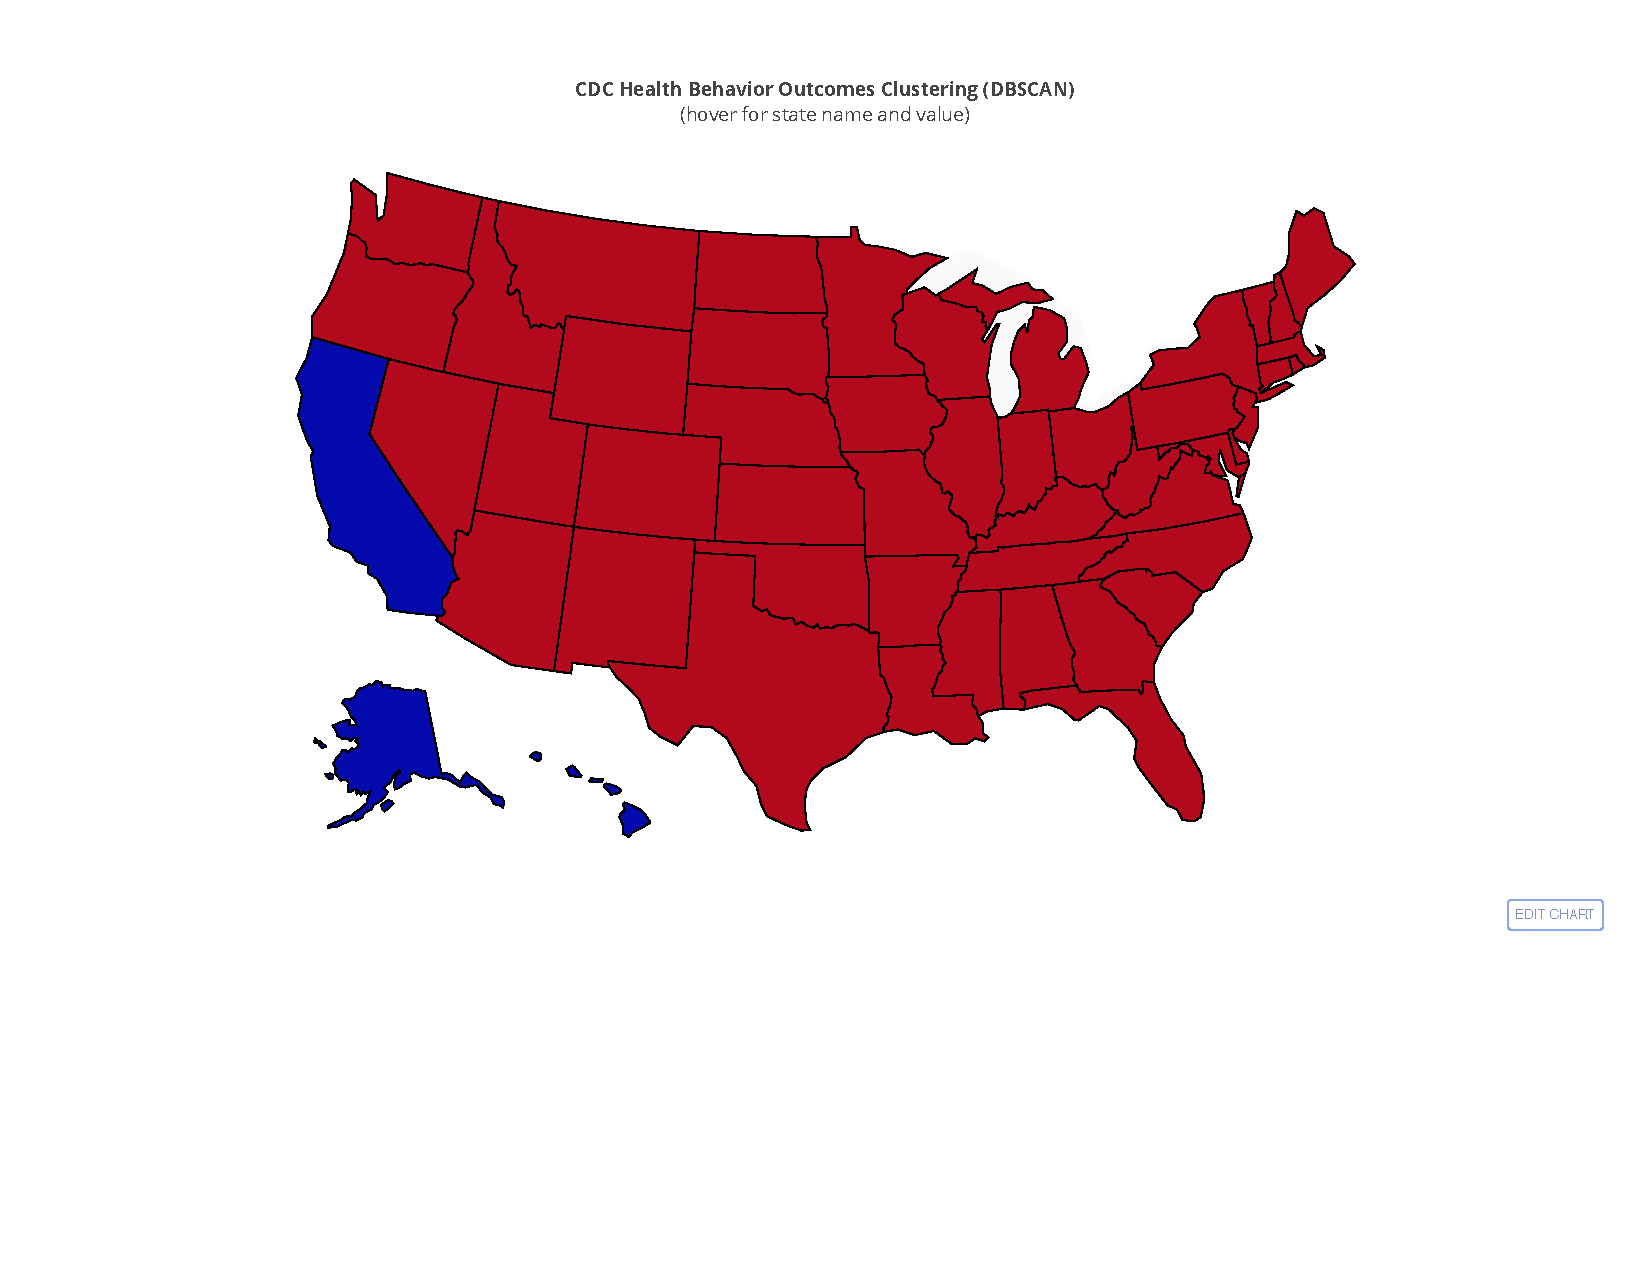
\includegraphics[width=\linewidth]{images/cdc_health_behavior_and_outcomes_dbscan_map.pdf}
\label{fig:dbhealthmap}
\end{figure}

\subsubsection{Hierarchical Clustering}
We then performed agglomerative hierarchical clustering using a Ward distance metric. The Ward metric was selected after comparing results from the single, complete, and average linkage metrics. This clustering is shown in \ref{fig:dbhealthdg}.

\begin{figure}[h]
\centering
\caption{}
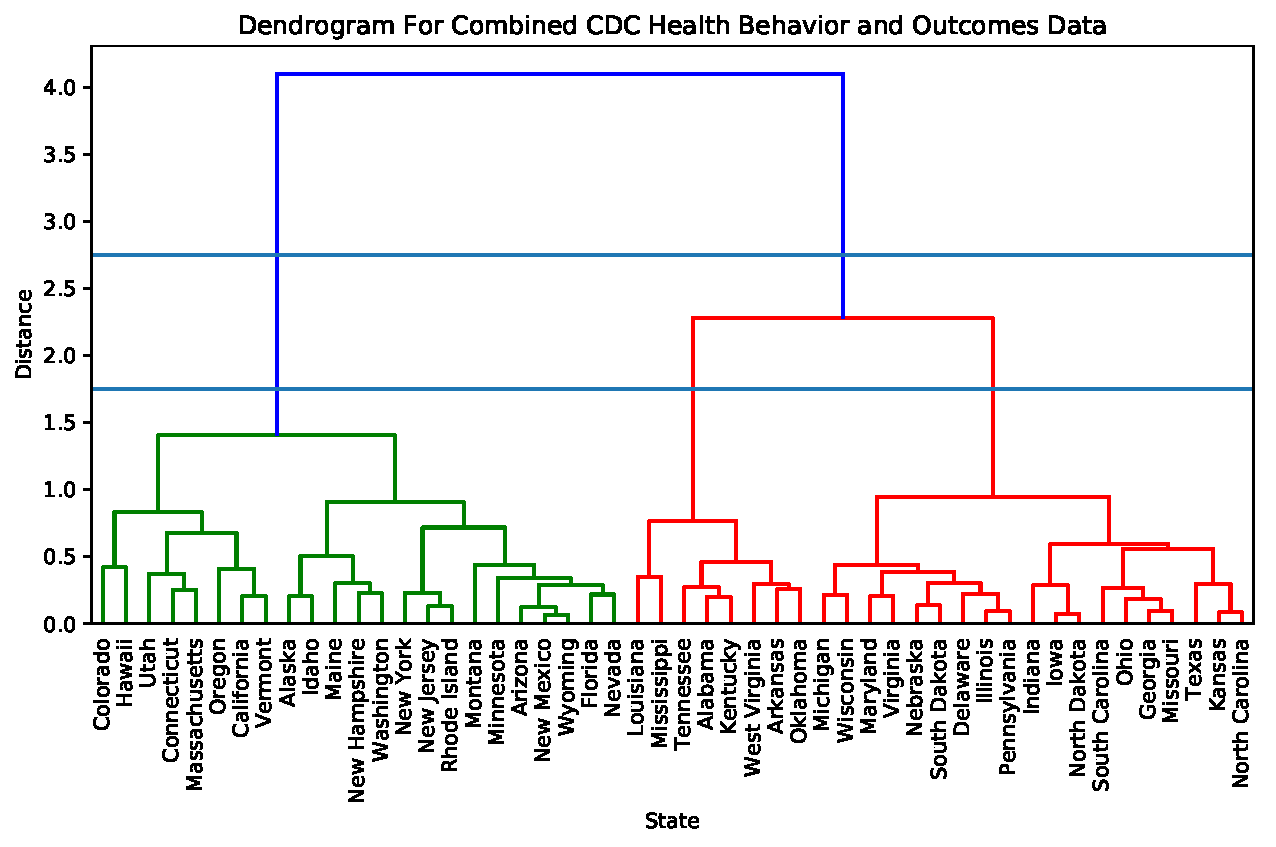
\includegraphics[width=\linewidth]{images/cdc_health_behavior_and_outcomes_agglomerative_dendrogram.pdf}
\label{fig:dbhealthdg}
\end{figure}

\section{Discussion}
\label{Discussion}
When visualized in two dimensions, cluster density appears to be relatively consistent which may explain the relatively poor performance of DBSCAN in finding separate clusters without classifying a large number of data points as noise. Cluster shape and size do not seem to vary too much to suggest problems with $k$-means clustering. However, in understanding these connections, the hierarchical clustering proved most useful as a dendrogram allowed for a clear visualization of the number of clusters and their respective distances. Looking at these clusters obtained through $k$-means and hierarchical clustering, these clusterings appear to follow geographical boundaries. For example, in the clustering of socioeconomic risk factor data: southern and midwest states (such as Louisiana, Mississippi, Alabama, Arkansas, Oklahoma) and coastal states (such as Connecticut, California, Massachusetts, Alaska, Hawaii) can be seen. When compared via the dendrograms obtained through hierarchical clustering, states that are most similar based on socioeconomic risk factors are often also similar in terms of health outcomes (for example, New York and Rhode Island). In the final project, we plan to more closely discuss these trends use metrics to compare the similarity of these groupings and identify states with similar socioeconomic risk factors but very different health behavior outcomes.

\begin{figure}[h]
	\centering
	\caption{Interpreting Principal Components- Socioeconomic Risk}
	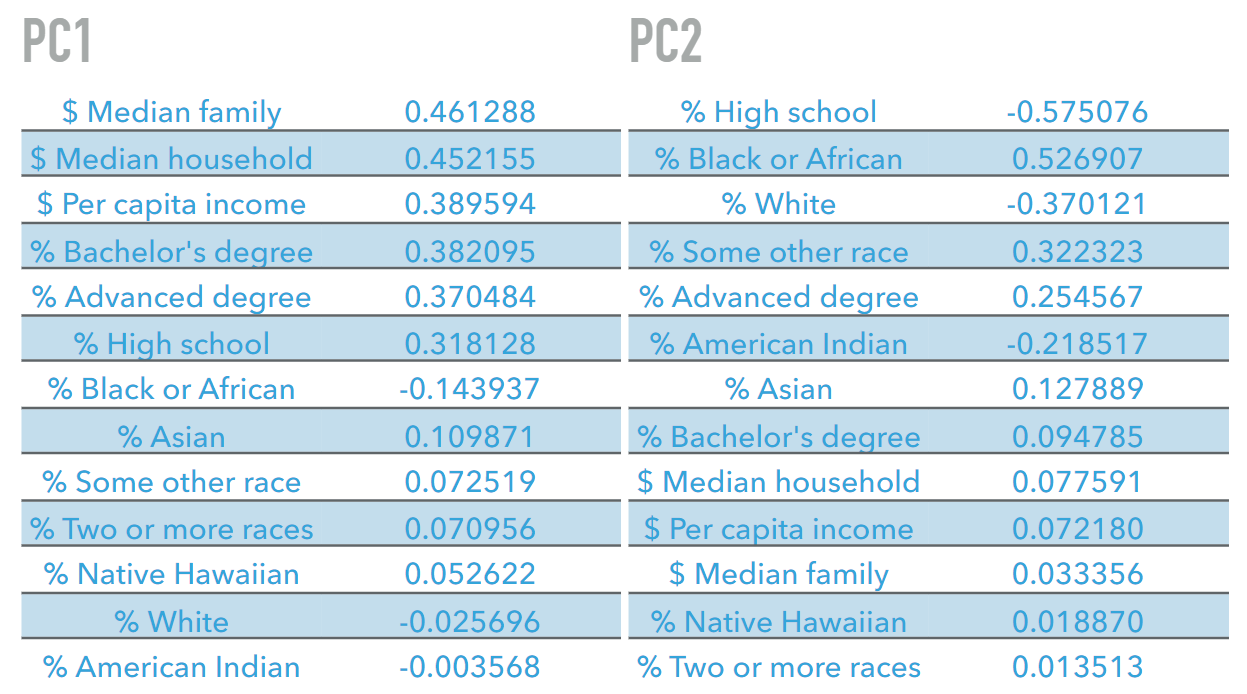
\includegraphics[width=\linewidth]{images/interpreting_pca_socioeconomic.png}
	\label{fig:pcaInterpretSocio}
\end{figure}

\begin{figure}[h]
	\centering
	\caption{Interpreting Principal Components- CDC Health Behavior}
	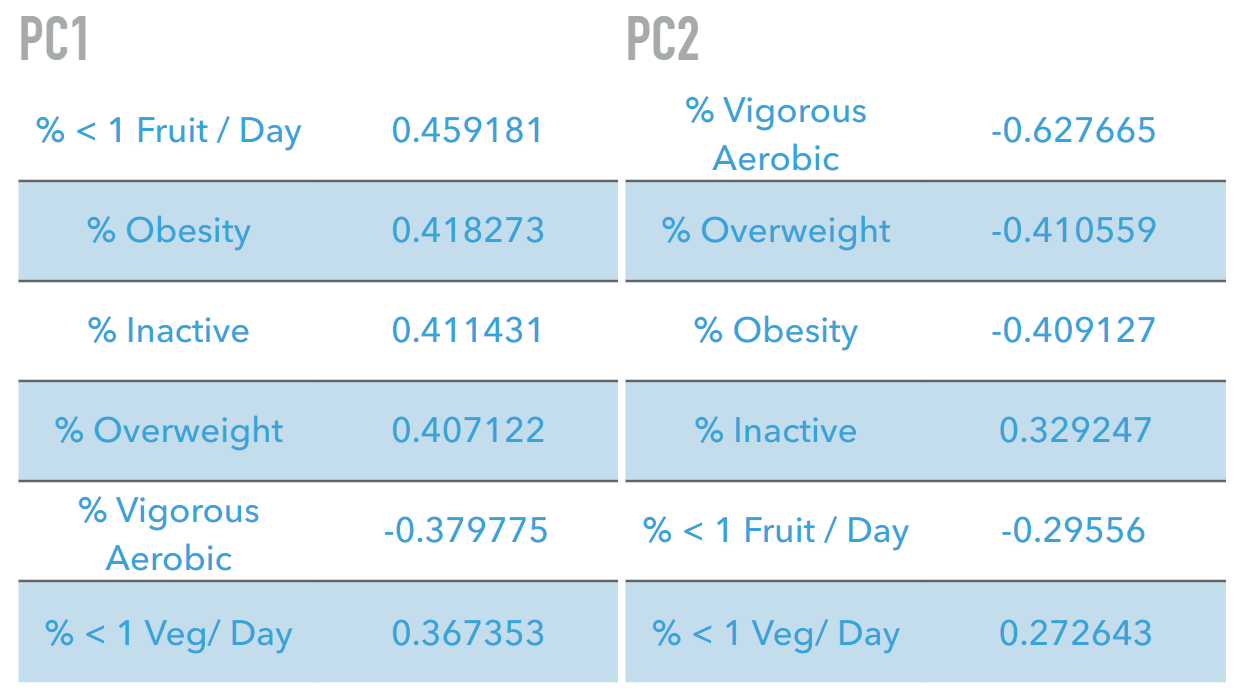
\includegraphics[width=\linewidth]{images/interpreting_pca_cdc.png}
	\label{fig:pcaInterpretCDC}
\end{figure}

\bibliography{report}
\bibliographystyle{icml2015}


\end{document} 


% This document was modified from the file originally made available by
% Pat Langley and Andrea Danyluk for ICML-2K. This version was
% created by Lise Getoor and Tobias Scheffer, it was slightly modified  
% from the 2010 version by Thorsten Joachims & Johannes Fuernkranz, 
% slightly modified from the 2009 version by Kiri Wagstaff and 
% Sam Roweis's 2008 version, which is slightly modified from 
% Prasad Tadepalli's 2007 version which is a lightly 
% changed version of the previous year's version by Andrew Moore, 
% which was in turn edited from those of Kristian Kersting and 
% Codrina Lauth. Alex Smola contributed to the algorithmic style files.  
